%%%%%%%%%%%%%%%%%%%%%%%%%%%%%%
%%%TFG
%%%%%%%%%%%%%%%%%%%%%%%%%%%%%%
\documentclass[12pt]{article}
%%%%%%%%%%%%%%%%%%%%%%%%%%%%%%
\usepackage[a4paper, margin = 24.5mm]{geometry}
\usepackage[utf8]{inputenc}
\usepackage[english,spanish]{babel}
\usepackage[hidelinks]{hyperref}
\usepackage{mathrsfs}
\usepackage{float} 
\usepackage{graphicx,anysize, geometry}
\usepackage{soul}
\usepackage{color,xcolor}
\usepackage{setspace}
\usepackage{amsmath}
\usepackage{amssymb}
\usepackage[utf8]{inputenc}
\usepackage{pdfpages}
\usepackage{graphicx}
\usepackage{subcaption}
\usepackage{pdfpages}
\usepackage{fancyhdr}
%%%%%%%%%%%%%%%%%%%%%%%%%%%%%%
\begin{document}
%%%%%%%%%%%%%%%%%%%%%%%%%%%%%%
%%% PORTADA
%%%%%%%%%%%%%%%%%%%%%%%%%%%%%%
\newgeometry{margin=1in}
\begin{titlepage}
\noindent\raisebox{0pt}[0pt][0pt]{

\includegraphics[width=10.5cm]{logo.pdf}}\par
\vspace{8.5cm}
    {\centering
    \scalebox{1.125}{\bfseries\sffamily\Huge Trabajo de Fin de Grado en Física}\par
    \rule{16.13cm}{1.5pt}\par
    \vspace{4.5cm}
    {\bfseries\sffamily\LARGE Introducción a la holografía digital en eje}\par
    }
\vfill
   {\raggedleft\sffamily
		Septiembre 2023\par
      \vspace{\baselineskip}
		Alumna: María Victoria Gómez Bifante\par
      \vspace{\baselineskip}
		Tutor (1): Genaro Saavedra Tortosa\par
		Tutor (2): Juan Carlos Barreiro Hervás\par
   }
\end{titlepage}
\restoregeometry
%%%%%%%%%%%%%%%%%%%%%%%%%%%%%%
%%% RESUMEN 
%%%%%%%%%%%%%%%%%%%%%%%%%%%%%%
\begin{abstract}
\textit{La holografía es una técnica de formación de imágenes tridimensionales que permite reconstruir el campo electromagnético trasmitido por un objeto a partir de registrar la intensidad de una interferencia. Sin embargo, en la técnica convencional, existe una  pérdida de información al recrear la imagen del objeto en ciertas configuraciones  dado que existe una superposición entre las componentes que forman el patrón de intensidad.  Ante la necesidad de solucionar las limitaciones de la técnica clásica y de extender así su funcionalidad a todos los tipos de configuración, nace el concepto de holografía digital. En este Trabajo de Fin de Grado se ha realizado un estudio teórico de la técnica holográfica, en particular, se ha verificado la solidez del modelo teórico de la holografía digital en eje. En primer lugar, se ha expuesto el mecanismo completo de la holografía clásica  para explicar así el efecto de la imagen gemela y  el solapamiento entre las componentes de la irradiancia en configuraciones en eje. A continuación,  se ha presentado la técnica holográfica  digital  y se ha desarrollado el procedimiento necesario tanto para eliminar el efecto de la imagen gemela como para dar solución a la problemática de la superposición entre las componentes de la intensidad. Por último, se ha llevado a cabo la simulación digital del mecanismo completo de la holografía en eje para recrear la imagen de dos objetos puros de fase que son invisibles con las técnicas de imagen convencionales.}
\end{abstract}
%%%%%%%%%%%%%%%%%%%%%%%%%%%%%%
%%% ABSTRACT
%%%%%%%%%%%%%%%%%%%%%%%%%%%%%%
\vspace{\baselineskip} 
\begin{otherlanguage}{english}\itshape
\begin{abstract}
Holography is a three-dimensional imaging technique that allows the reconstruction of the electromagnetic field transmitted by an object after recording the intensity of an interference. However, there is a loss of information when the image is reconstructed in some setups because there is an overlap between the components that form the intensity pattern. Digital holography is created to solve the problem of overlapping and to extend its functionality to all configurations. In this bachelor's project a study of  the  holographic technique, in particular, the solidity of the theoretical model of on-axis digital holography is verified. First, the complete mechanism of classical holography has been exposed.
The reason of this  is to explain the twin image effect and expose the problem of overlap between the irradiance components in on-axis setups. Next, the digital holographic technique has been presented and  has been developed  to eliminate the twin image effect and to solve the problem of overlapping between the intensity components. To finish, the on-axis digital holography mechanism has been simulated to recreate the image of two pure phase objects that are invisible with conventional imaging technique.
\end{abstract}
\end{otherlanguage}
%%
\newpage
\tableofcontents
\newpage
\pagestyle{fancy}
\lhead[Trabajo de Fin de Grado en Física]{Trabajo de Fin de Grado en Física}
\rhead[Septiembre 2023]{Septiembre 2023}
%%%%%%%%%%%%%%%%%%%%%%%%%%%%%%
%%% INTRODUCCIÓN 
%%%%%%%%%%%%%%%%%%%%%%%%%%%%%%
\section{Introducción}
La técnica holográfica es un proceso que permite almacenar la información sobre la distribución del campo electromagnético resultante de una interferencia, para posteriormente  reconstruir a partir de ella, la distribución del campo  trasmitido por un objeto concreto. Tras recrear el campo luminoso  que emerge del mismo, el observador puede visualizar la imagen  tridimensional del objeto. \\ \\ 
%%%
A diferencia de las técnicas convencionales de formación de imágenes que únicamente permiten extraer la amplitud de la  distribución del campo emitido por el objeto, como es el caso de la fotografía, la holografía permite obtener tanto la amplitud como fase. Dicha información se puede almacenar mediante la interferencia entre una onda emergente del objeto con otra onda utilizada de referencia, y a partir de ella, se puede extraer la amplitud y la fase de la onda trasmitida por el objeto. Dado que esta amplitud y esta fase se replican exactamente como si emergieran del propio objeto, otorgan tridimensionalidad a la imagen.\\ \\
%%%
El concepto de la holografía surge con las pioneras investigaciones de Dennis Gabor \cite{1} en el año 1948. Su primer montaje, conocido como  configuración en eje,  resultó sufrir una pérdida de información al registrar el patrón de intensidad de la interferencia. Posteriormente, en el año 1964,  Emmett Leith y Juris Upatnieks \cite{2} fueron quienes idearon un nuevo montaje conocido como configuración fuera de eje. En ambos casos se requería de una fuente espacialmente coherente y monocromática para  desarrollarse experimentalmente. Por ese motivo no fue  hasta  la aparición del láser, en la década de los 60, que pudieron llevarse a la práctica. \\ \\
%%%
Del refinamiento de las técnicas holográficas convencionales  y ante la necesidad de solucionar la pérdida de información en las configuraciones en eje, nace el concepto actual de la holografía digital. Dicha evolución es el resultado de aplicar sobre el concepto clásico de holografía,  tanto los métodos actuales para el tratamiento de datos como las técnicas computacionales más avanzadas. A diferencia de la técnica holográfica  convencional, la holografía digital permite extraer  la  información  de  la distribución del campo electromagnético emergente del objeto de una manera más directa. Por lo que las diferenciamos  en el método de registro, en la capacidad de modificar, de extraer y también de reconstruir, la información de la interferencia.  Además, esta técnica permite tomar medidas cuantitativas como la profundidad del objeto, dado que los mapas reconstruidos están digitalizados. Por lo tanto, la holografía digital es un mecanismo válido para todos los tipos de configuración ya que no tiene las restricciones que sí presentaba la holografía clásica.\\ \\ 
%%%
En primer lugar, clasificaremos el mecanismo de la holografía en la etapa de registro y en la etapa de reconstrucción. La etapa de registro corresponde a la captura del patrón de intensidad  de una interferencia, mientras que la etapa de reconstrucción regenera la distribución de amplitud del campo  transmitido por el objeto a partir de la intensidad registrada. A continuación, expondremos los fundamentos teóricos   de la holografía clásica para posteriormente,  registrar e interpretar la información del patrón intensidad  para el caso de una interferencia entre dos ondas planas. Después,  detallaremos  el proceso para recrear la imagen tridimensional del objeto e interpretaremos todos los campos luminosos que se reconstruyen junto a ella y por ende,  explicaremos el efecto visual de la imagen gemela. Dado que en los montajes en eje existe un solapamiento entre las componentes del patrón de intensidad, estas se reconstruirán ópticamente sobre el mismo eje y por consiguiente, perderemos información al recrear la imagen del objeto.\\ \\
%%%
Después, expondremos los fundamentos  de la holografía digital y explicaremos tanto el proceso de registro como los cálculos digitales empleados para generar el campo luminoso tridimensional emergente del objeto. Además, utilizaremos la holografía digital para suprimir  la reconstrucción de las componentes que puedan perturbar la visualización de la imagen, de modo que también eliminaremos el efecto de la imagen gemela. Por lo tanto,  la técnica holográfica digital permite  mejorar  la calidad de la imagen reconstruida. \\ \\
%%%
Desde la holografía digital, presentaremos la técnica de filtrado y el método de variación de fase como los procesos más comunes para recrear la imagen del objeto sin perturbaciones visuales. Por un lado, transformaremos  el patrón de intensidad  al espacio de Fourier con el objetivo de  separar sus componentes   inicialmente solapadas para después,  volver al dominio espacial y filtrar la componente  que queremos reconstruir. Por otro lado, recrearemos únicamente la imagen tridimensional del objeto a partir de estudiar  la dependencia del patrón de intensidad con  la variación de fase de la onda trasmitida por el objeto. \\ \\
%%%
Para finalizar nuestro estudio, verificaremos la eficacia del método de variación de fase en configuraciones en eje a partir de simular digitalmente el proceso  para reconstruir la distribución de amplitud del campo emitido por un objeto. Concretamente, simularemos la reconstrucción de dos objetos de fase: uno de fase constante sobre un fondo uniforme  y otro con variación lineal de fase desde el centro hasta el borde.
%%%%%%%%%%%%%%%%%%%%%%%%%%%%%%
%%% HOLOGRAFÍA CLÁSICA 
%%%%%%%%%%%%%%%%%%%%%%%%%%%%%%
\section{Holografía clásica}
La holografía clásica es una técnica de formación de imágenes que consiste en reconstruir la distribución de onda electromagnética asociada al campo luminoso emergente de un objeto  a partir del registro  de una interferencia. Al añadir una onda como referencia y provocar su incidencia con otra de las mismas características pero  trasmitida por el objeto  sobre una placa fotográfica, llamada holograma analógico, se consigue grabar la información cifrada de la interacción en amplitud y en fase.  \\ \\
%%
Un holograma analógico\footnote{En esta sección del trabajo, se hará referencia al holograma analógico únicamente  como holograma.} es un elemento óptico de transmitancia en amplitud definida  $t(\Vec{x})$ que permite capturar o grabar el patrón de intensidad de una interferencia entre  dos frentes de onda. El patrón de intensidad almacenado en la $t(\Vec{x})$  del holograma, contiene la información codificada de la interferencia en un instante determinado. Al descodificarla, se puede extraer tanto la amplitud como la fase del frente de ondas que se quiere reconstruir. Si después, se ilumina $t(\Vec{x})$ con una fuente de  características similares a la onda usada como referencia, se puede reconstruir el campo luminoso trasmitido por el objeto. Por lo tanto, es posible recrear  la imagen tridimensional del objeto a partir de grabar el patrón de intensidades  en la $t (\vec{x})$ del holograma. Es conveniente destacar que existen diferentes tipos de hologramas y montajes para capturar la interferencia en $t (\vec{x})$, pero centraremos nuestro estudio en el registro del holograma por trasmisión\footnote{Los hologramas por trasmisión capturan el patrón de intensidad de una interferencia  cuando la interacción entre ondas cae directamente sobre el lado de emulsión de la placa fotográfica. Se puede ampliar su descripción junto con la de otros tipos de hologramas en  \cite{4}.}. \\ \\
%%%
Para entender el concepto de la holografía \cite{5}, comenzamos clasificando el proceso en la etapa de registro y en la etapa de reconstrucción según se almacene o se analice la información capurada en el holograma. \\ \\
%%%
Veamos con más detalle la etapa de registro. Definimos el eje $OZ$ como el eje óptico transversal al plano  $XY$. A una distancia axial $z$ del origen de $OZ$, registramos un holograma  descrito en $\Vec{x} = (x, y)$. De la misma manera,  colocamos el objeto en $z = 0$ desplazado transversalmente e iluminado con una onda plana propagante en un ángulo $\theta$ del eje $OZ$ respecto al plano $XZ$.  Después, iluminamos el sistema con una fuente  de luz $\mathbb{F}$ de la que emerge una onda plana con longitud de onda definida $\lambda$ coherente con el haz objeto. En la práctica, ambos haces provienen en realidad de la misma fuente $\mathbb{F}$. Así, provocamos la interacción  del frente de ondas de $\mathbb{F}$ con otro de la misma procedencia pero transmitido por el objeto.  Si guiamos  la superposición entre estos dos frentes de onda coherentes para que ocurra sobre el plano del holograma\footnote{El plano del holograma es el plano bidimensiomal sobre el que se coloca el holograma. Dicho plano se sitúa  a una distancia axial $z$ sobre el eje óptico $OZ$ y  se describe espacialmente en $\Vec{x}$.},   transferiremos la información  de la interacción como intensidad  a  su transmitancia $t(\vec{x})$. Entendemos como intensidad o irradiancia al flujo del campo electromagnético  por  unidad de superficie del plano transversal sobre el que se describe.  Por tanto, $t(\vec{x})$ contendrá la información codificada, en amplitud y en fase, de las  distribuciones de onda capturadas sobre el plano del holograma.  \\ \\
%%%
 A cada uno de los frentes de onda partícipes en la interferencia, le asignamos   una  distribución de amplitud compleja del campo electromagnético. Previamente a definirlas, buscamos que tengan  una representación en todo el dominio espacial y para ello, limitamos su difracción\footnote{En en este caso,  la difracción se entiende como la propagación  de la distribución  de amplitud compleja del campo electromagnético. Se utilizarán los conceptos de propagación y difracción de forma indistinta.} a distancias cercanas al eje óptico $OZ$ con la aproximación paraxial. De esta manera, la distancia axial desde  un punto inicial $\Vec{r_0} = (x_0, y_0, z_0)$ del objeto hasta un punto $\vec{r} = (x, y, z)$  sobre el holograma, será mucho mayor a la suma cuadrática de las distancias transversales, es decir, las distribuciones de onda deben verificar $(x-x_0)^2 + (y-y_0)^{2} \ll (z - z_0)^2$. Simplificaremos también, el comportamiento de la propagación de las distribuciones de onda con la teoría escalar de la difracción,  ya que dicha simplificación  nos permite omitir el caracter vectorial  de las ondas electromagnéticas cuando la distancia de observación es lo suficientemente grande.  Podemos encontrar la demostración de ambas consideraciones  en \cite{6}. Además, se trata de un sistema lineal por lo que la propagación libre de la luz es invariante  ante desplazamientos transversales en el espacio libre.  Por lo que si interpretamos la integral de la difracción como  la convolución\footnote{El operador convolución $\circledast$ se define como $f(\Vec{x}) \circledast g(\Vec{x}) = \int \int f(\Vec{\alpha})g(\Vec{x}- \Vec{\alpha})d^{2}\vec{\alpha}$. Es el resultado de la superposición de $f(\Vec{\alpha})$ sobre una versión de $g(\Vec{\alpha})$ trasladada e invertida $g(\Vec{x}-\Vec{\alpha})$, de modo que  transforma dos funciones bidimensionales en una tercera. Se detalla el producto de la convolución para la óptica paraxial propia  de la difracción de Fresnel  en  \cite{7}.} entre una distribución de amplitud del campo transversal en la posición inicial y la respuesta impulsional $h(\Vec{x}, z)$  asociada a la propagación libre, podemos regenerar el mismo campo  a una distancia axial $z$ sobre el eje $OZ$.  Dicho de otro modo, podemos reconstruir la distribución de amplitud del campo difractado en todos y cada uno de los planos transversales $XY$ a lo largo del eje $OZ$. A su vez, entendemos como  respuesta impulsional\footnote{Se puede comprobar en  \cite{8} que la propagación libre es invariante ante desplazamientos  transversales, de  manera que la respuesta impulsional  $h (\Vec{x}, z)$ queda simplemente desplazada  $h (\Vec{x} - \Vec{x_0}, z - z_0)$.} a la función   $h(\Vec{x}, z)$   que representa la distribución del campo electromagnético en un plano $XY$ situado sobre el eje óptico a una distancia $z$ de una fuente puntual sobre el eje óptico.\\ \\
%%%
Comenzamos definiendo al frente de ondas difractado por el objeto desde $z = 0$ hasta $z$ sobre el plano del holograma como  la distribución de amplitud compleja $U_O (\vec{x}, z)$ de intensidad  $I_O(\Vec{x}, z) = {\mid}U_O (\Vec{x}, z){\mid}^{2}$.  Tal y como hemos visto, determinamos la distribución de onda  $U_O (\vec{x}, z)$ aplicando la convolución entre  la distribución de amplitud del campo  inicial   y  la respuesta impulsional  $h (\Vec{x}, z)$. Si concretamos  la respuesta impulsional para $h (\Vec{x}, z)= e^{i \frac{\pi}{z \lambda} \mid \vec{x} \mid ^{2}}$, la descripción de  $U_O (\vec{x}, z)$  en el plano de la interferencia  es
%%%
\begin{equation}
    U_O (\vec{x}, z) =  U_O (\vec{x}, 0) \circledast e^{i \frac{\pi {\mid \vec{x} \mid}^{2}}{z \lambda}},
    \label{Ec.1}
\end{equation}
%%%
donde $U_O (\Vec{x}, 0)$ es la distribución  de amplitud del campo  inicial descrito en el origen de $OZ$ y $\circledast$ representa la operación de convolución.\\ \\
%%%
El frente de onda del objeto  se genera al iluminar dicho objeto con una onda plana procedente de la fuente $\mathbb{F}$. Si suponemos que iluminamos el objeto con una onda plana inclinada un ángulo $\theta$ respecto el eje óptico  y escogemos los ejes de referencia de forma que la dirección de propagación  de esta onda plana sea $\hat{s}_O \equiv (\sin{\theta}, 0, \cos{\theta})$, podemos factorizar el frente de onda del objeto como
%%%
\begin{equation}
    U_O (\vec{x}, 0) =  A_O (\vec{x}, 0) e^{i k x \sin{\theta}},
    \label{Ec.2}
\end{equation}
%%%
siendo $k = \frac{2 \pi}{\lambda}$ el número de ondas de la iluminación procedente de $\mathbb{F}$ y  $A_O (\vec{x}, 0)$ la transmitancia en amplitud del objeto.\\ \\
%%%
Si propagamos esta distribución de amplitud  hasta el plano del holograma, describiremos el frente de onda del objeto como
%%%
\begin{equation}
    U_O (\vec{x}, z) =  A_O (\vec{x}, z) e^{i k (x \sin{\theta} + z \cos{\theta})},
    \label{Ec.3}
\end{equation}
%%%
donde $A_O (\vec{x}, z)$ corresponde al patrón de difracción del objeto a una distancia $z$ respecto al origen de $OZ$.\\ \\
%%%
A su vez, definimos al  frente de ondas plano emergente de  $\mathbb{F}$ como la distribución de amplitud compleja $U_R (\vec{x}, z)$ de intensidad constante $I_R(\vec{x}, z) = {\mid}U_R (\Vec{x}, z){\mid}^{2}$. Describimos la propagación axial de $U_R (\vec{x}, z)$ con el vector de propagación $\Vec{k} = \frac{2 \pi}{\lambda} (0, 0, \hat{z})$. Por tanto, la distribución de amplitud asociada a la propagación del haz de referencia, en el plano del holograma, viene dada por
%%%
\begin{equation}
    U_R (\vec{x}, z) = e^{i k z}.
    \label{Ec.4}
\end{equation}
%%%
Por simplicidad, hemos consideramos  la amplitud como la unidad, por lo que $I_R(\Vec{x}, z) = 1$. \\ \\
%%%
Después de definir  las ondas sobre el plano del holograma, representamos su propagación  en el espacio libre como haces perpendiculares a las superficies  de sus respectivos  frentes de onda. Por ello, nos referimos  a la propagación de la distribución de amplitud trasmitida por el objeto como \textbf{haz objeto} y de la misma manera, llamamos \textbf{haz de referencia} a la propagación la distribución de amplitud emergente de $\mathbb{F}$. La interacción entre ambos haces  ocurre en el holograma y por ello, la información de la interferencia entre  $U_O (\Vec{x}, z)$ y $U_R (\Vec{x}, z)$ queda almacenada  en la transmitancia $t(\Vec{x})$  del holograma. \\ \\
%%%
Suponemos que nuestro  holograma es una placa fotosensible ideal, por lo que su transmitancia en amplitud registrará la información de la intensidad sin perder información en el revelado, de modo que consideramos  $t(\Vec{x}) \sim  I (\Vec{x}, z)$. Como la intensidad  es proporcional al módulo al cuadrado de la distribución de amplitud resultante de la  superposición  $U_O (\Vec{x}, z) + U_R (\Vec{x}, z)$, tras el registro,  la irradiancia  de la interferencia  queda almacenada en la transmitancia en amplitud como 
%%%
\begin{equation}
     I (\Vec{x}, z) =  \mid  U_O (\Vec{x}, z) + U_R (\Vec{x}, z) \mid  ^{ 2 }.
     \label{Ec.5}
\end{equation}
%%%
Por consiguiente,  la forma extendida de la intensidad de la Ec.(\ref{Ec.5}) viene dada por
%%%
\begin{equation}
      I (\Vec{x}, z) =  \mid  U_O (\Vec{x}, z) \mid ^{2} +  \mid U_R (\Vec{x}, z) \mid ^{2} + U_O (\Vec{x}, z) U_R^{*} (\Vec{x}, z) + U_R (\Vec{x}, z) U_O^{*} (\Vec{x}, z),
    \label{Ec.6}
\end{equation}
%%%
cuyo símbolo $\ast$ representa las distribuciones de amplitud complejas conjugadas $U_R^{*}(\Vec{x}, z)$ y $U_O^{*} (\Vec{x}, z)$  asociadas al haz de referencia y al haz objeto, respectivamente. \\ \\
%%%
Después, sustituimos  en la Ec.(\ref{Ec.6}) las definiciones de la Ec.(\ref{Ec.3}) y de la Ec.(\ref{Ec.4}) y obtenemos
%%%
\begin{align}
     I (\Vec{x}, z) =&  \mid A_O (\Vec{x}, z) \mid ^{2} + 1 + A_O (\Vec{x}, z) e^{i k (x \sin{\theta}+ z\cos{\theta})} e^{- i k z} \nonumber \\
     &+ A_O^{*} (\Vec{x}, z) e^{- i k (x \sin{\theta} + z \cos{\theta})} e^{i k z}.
    \label{Ec.7}
\end{align}
%%%
Por un lado, la primera componente  representa la  intensidad   $I_O(\Vec{x}, z)$ de la distribución de amplitud del campo emitido por el objeto, mientras que por otro, interpretamos al segundo término como la irradiancia  $I_R(\Vec{x}, z)$ de la distribución de amplitud asociada a la propagación del haz de referencia. Al resto, lo definimos como  término cruzado y expone la relación entre $U_O (\vec{x}, z)$ y $U_R (\vec{x}, z)$. Además, el factor de fase  $e^{\pm i k (x \sin{\theta} + z \cos{\theta})}$  muestra una  relación entre la interferencia con  el ángulo interferencial $\theta$.\\ \\
%%%
Esquematizamos la etapa de registro de nuestro sistema en la Fig.\ref{figura1}. Observamos como el frente de ondas procedente de la fuente incide sobre una lámina semiespejada. Dicha lámina está orientada de tal manera que  divide el frente  en dos, formando un ángulo $\pi/2$ entre sí. A continuación,  cada uno de los frentes se propaga hasta incidir sobre un espejo para cambiar su dirección. Por un lado, generamos el frente de ondas objeto al iluminar nuestro objeto, colocado en $z=0$  sobre el plano $XZ$,  con uno de los frentes de ondas plano y lo propagamos hasta una lámina semiespejada orientable. Por otro lado, vemos que el haz restante incide sobre la misma lámina semiespejada orientable. La orientación de la lámina provoca que el haz de referencia continue su propagación sin desviarse hasta caer sobre la superficie del holograma, mientras que el haz objeto caerá sobre el holograma con un ángulo $\theta$ respecto $OZ$ en el plano $XZ$.
%%%
\begin{figure}[bt!]
    \centering
    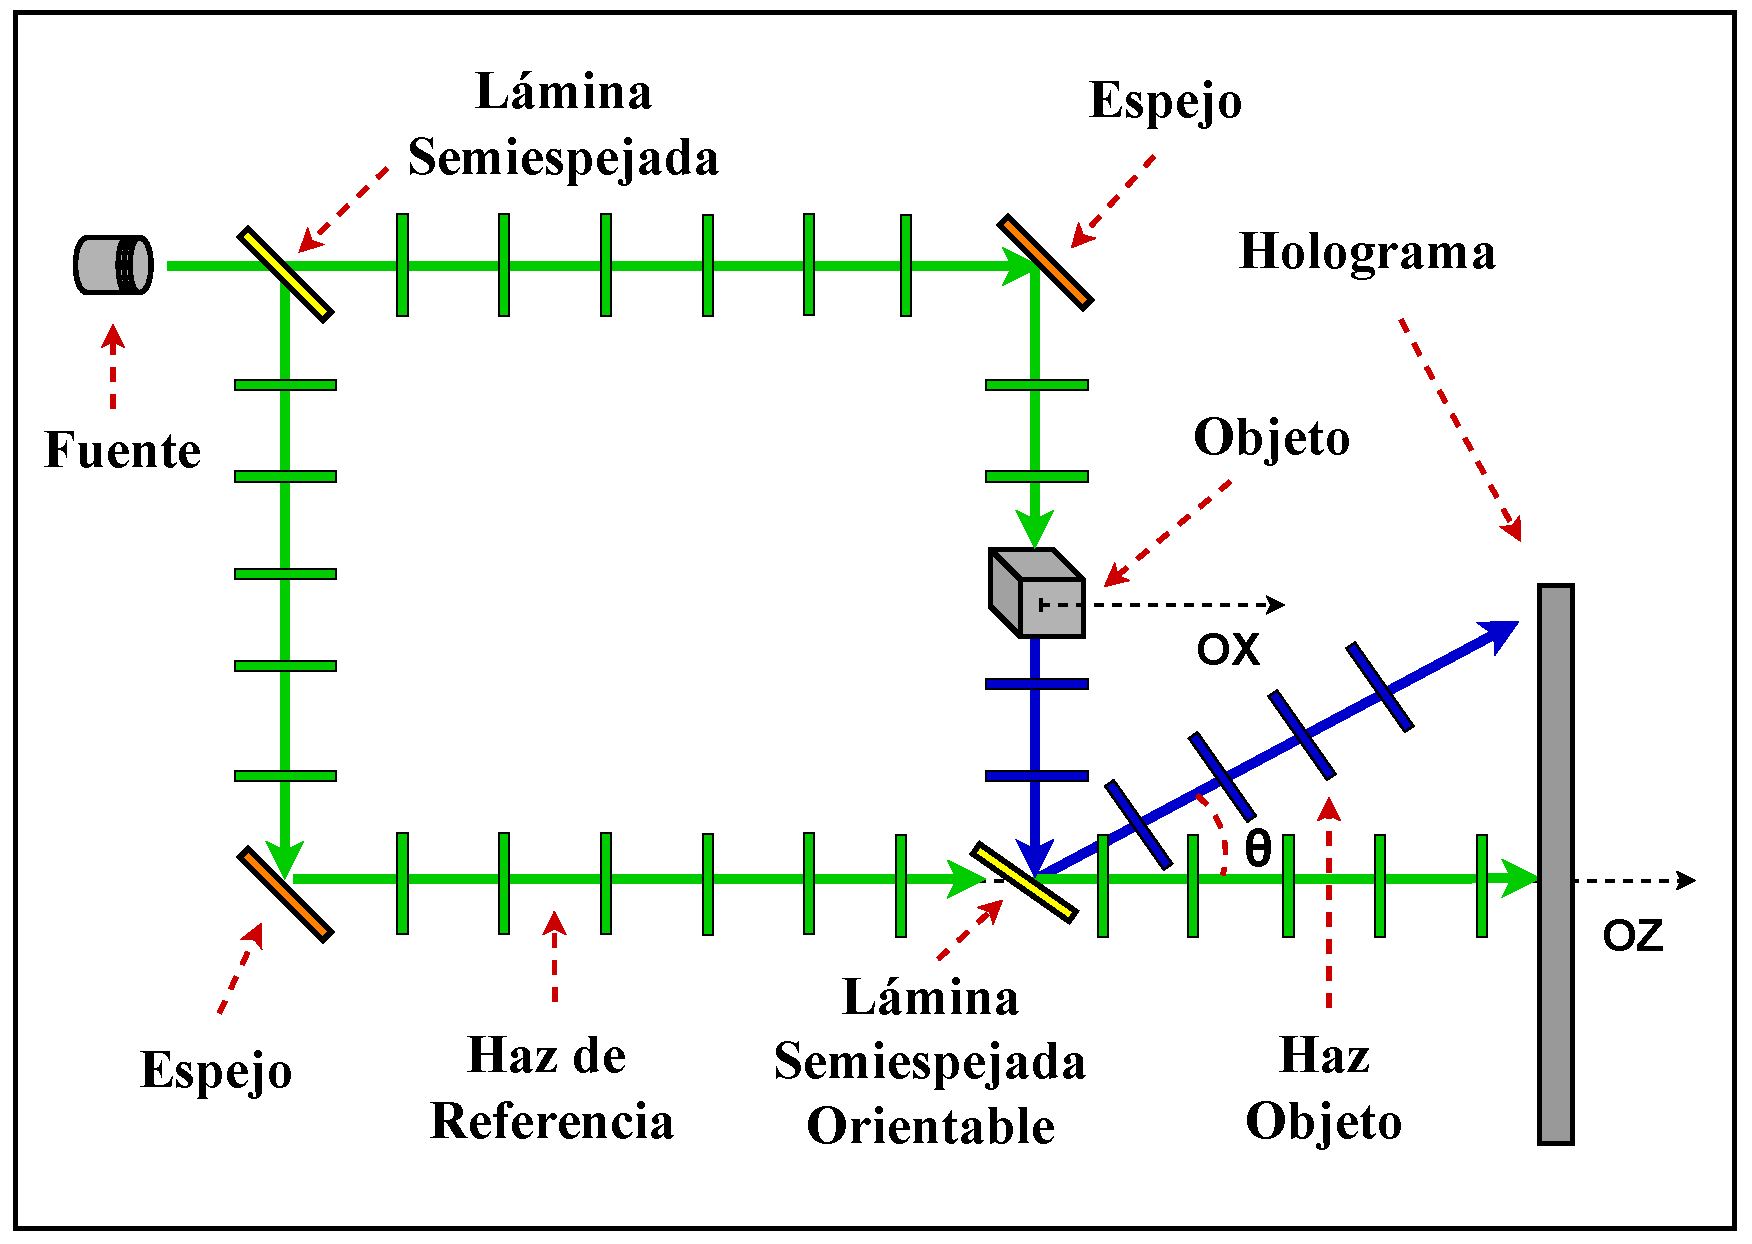
\includegraphics[scale = 0.4]{figure_1.pdf}\\
    \caption{Etapa de registro  para una configuración fuera de eje.}
    \label{figura1}
\end{figure}
%%%
A este tipo de montaje lo conocemos como configuración fuera de eje y corresponde al ideado por   Emmett Leith y Juris Upatnieks. \\ \\
%%%
Si ajustamos la orientación de la última lámina semiespejada para que el frente de ondas objeto y el frente de ondas de referencia se propagen de forma cuasi paralela hasta incidir sobre el holograma, estamos ante la configuración en eje de Gabor. En la Fig.\ref{figura2}, esquematizamos la etapa de registro cuando $\theta \sim 0$.
%%%
\begin{figure}[bt!]
    \centering
    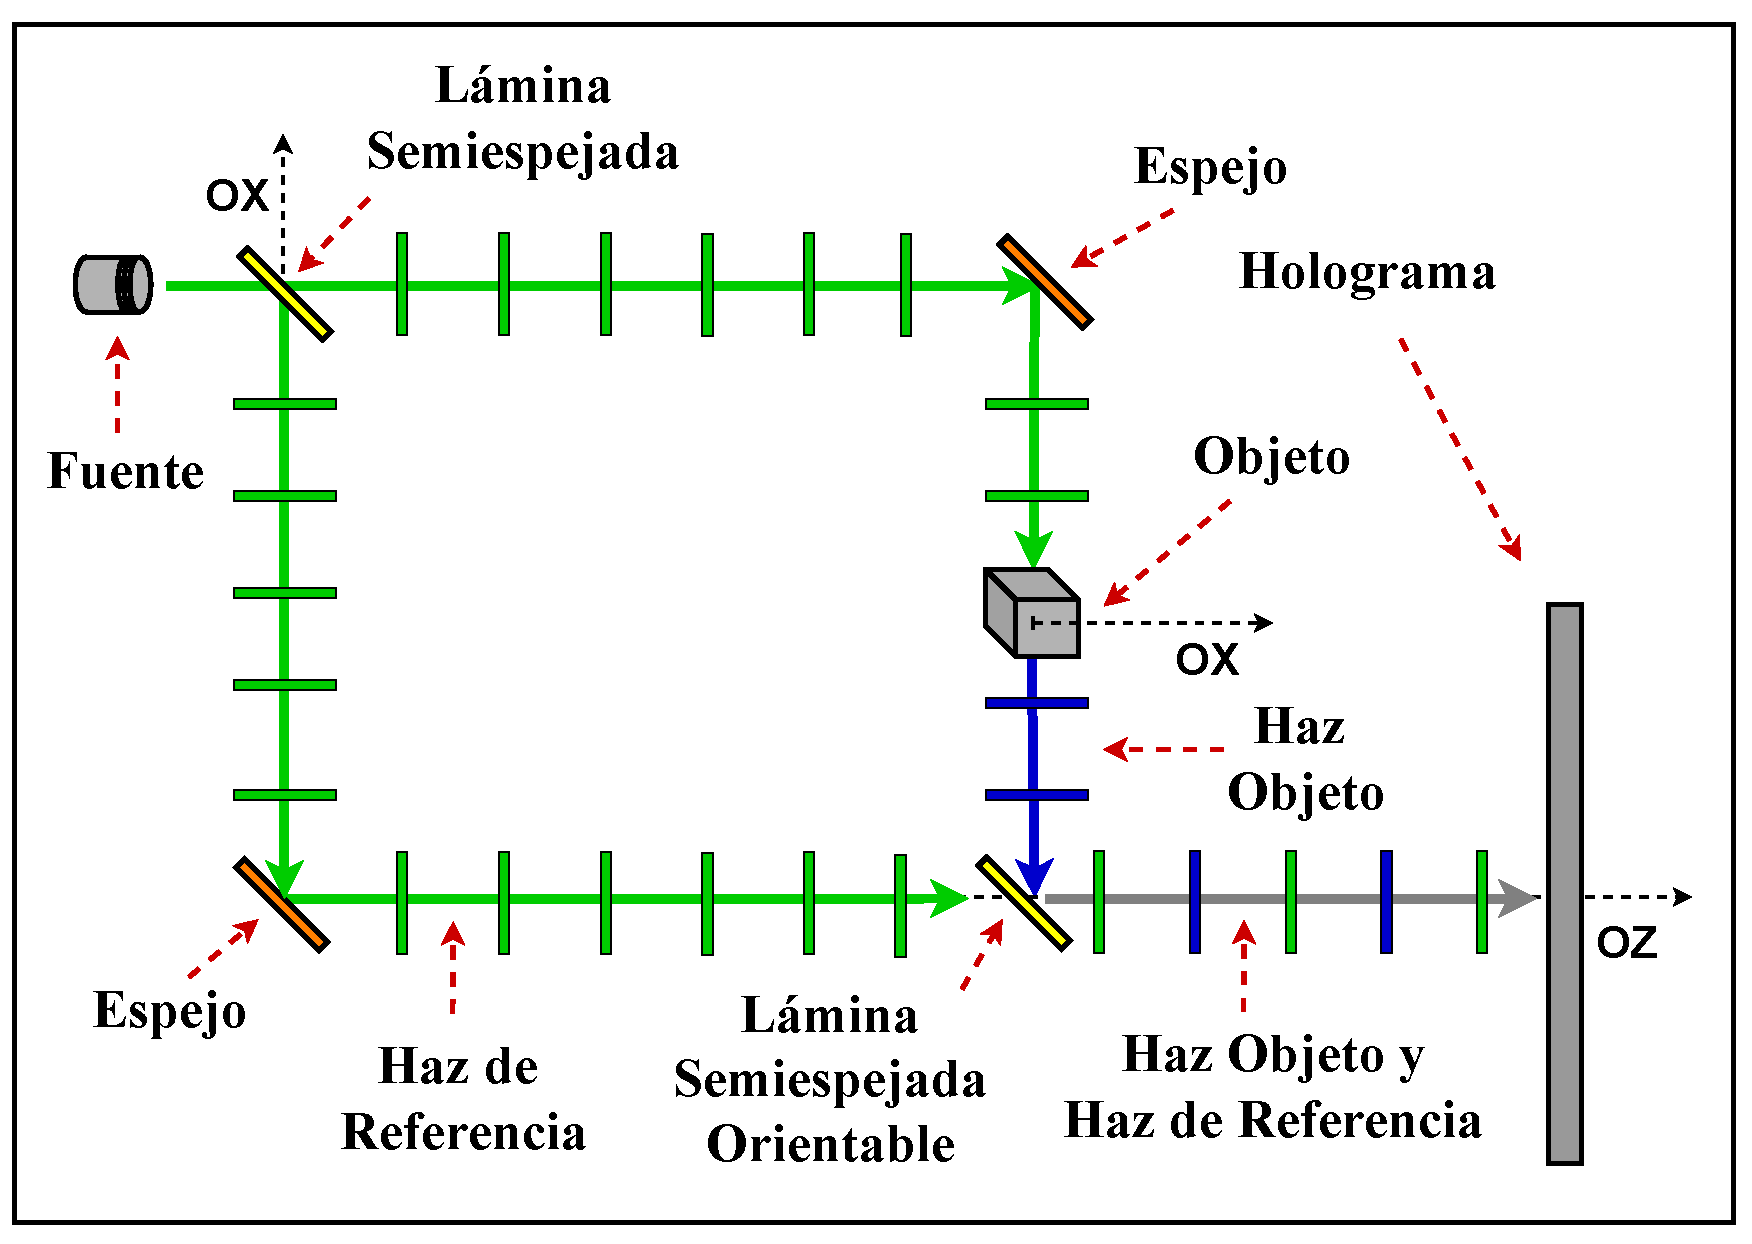
\includegraphics[scale = 0.4]{figure_2.pdf}\\
    \caption{Etapa de registro para una configuración en eje.}
    \label{figura2}
\end{figure}
%%%
Una vez hemos codificado la información de la interferencia en la $t (\vec{x})$ del holograma, damos por finalizada la etapa de registro.  \\ \\
%%%
Veamos ahora la etapa de reconstrucción. Nuestro objetivo es analizar el patrón de interferencia previamente registrado en el holograma para extraer de él, la información necesaria para recrear la imagen tridimensional del objeto.  Por ese motivo, buscamos aislar la distribución de amplitud $ U_O (\Vec{x}, z)$ en un término independiente a partir de la Ec.(\ref{Ec.7}) inicialmente mezclada. \\ \\
%%%
En primer lugar, volvemos a iluminar el holograma con un haz emergente de la fuente  $\mathbb{F}$ con distribución de amplitud compleja de características similares al haz de referencia. Por comodidad, en esta etapa, nos referimos  a este nuevo frente de ondas como  \textbf{haz de referencia}. \\ \\ \\
%%%
Después de reiluminar $t(\Vec{x})$,  la distribución de amplitud difractada a través del holograma  viene dada por
%%%
\begin{equation}
    U(\Vec{x}, z) = e^{ i k z} t (\Vec{x}).
    \label{Ec.8}
\end{equation}
%%%%
Dado que $t (\Vec{x}) \sim I (\Vec{x}, z)$,  sustituimos  la intensidad de la Ec.(\ref{Ec.7}) en  la Ec.(\ref{Ec.8}). Así, obtenemos la distribución de amplitud  de la Ec.(\ref{Ec.8}) como
%%%
\begin{align}
     U(\Vec{x}, z)=&  e^{i k z}  \left( \mid A_O (\Vec{x}, z) \mid ^{2} +  1 \right) +  A_O (\Vec{x}, z) e^{i k (x \sin{\theta}+ z\cos{\theta})} \nonumber \\
     &+ A_O^{*}(\Vec{x}, z) e^{- i k (x \sin{\theta}+ z\cos{\theta})} e^{ 2 i k z}.
      \label{Ec.9}
\end{align}
%%%
 Los dos primeros términos representan el haz incidente sobre $t(\Vec{x})$ modulado por la suma de las irradiancias del haz objeto y del haz de referencia respectivamente, es decir, simbolizan $e^{i k z} I_O (\Vec{x}, z) +  e^{ i k z} I_R (\Vec{x}, z)$ para  $I_O (\Vec{x}, z) = \mid A_O (\Vec{x}, z) \mid ^{2}$ y $I_R (\Vec{x}, z) = 1$. A su vez, las dos últimas componentes corresponden a la modulación del término cruzado con el nuevo haz de referencia.  Por simplicidad, ignoraremos en adelante los factores que únicamente dependen de $z$, ya que son contantes en el plano del holograma y no afectan al razonamiento posterior.\\ \\
 %%%
 Finalmente,  la distribución de amplitud  $U(\Vec{x}, z)$ resultante de la reiluminación del holograma  viene dada por
 %%%
 \begin{equation}
    U(\Vec{x}, z) = I_O (\Vec{x}, z) +  1 +  A_O (\Vec{x}, z) e^{i k x \sin{\theta}} +  A_O^{*} (\Vec{x}, z)  e^{- i k x \sin{\theta}}.
    \label{Ec.10}
\end{equation}
%%%
La primera componente de $U (\Vec{x}, z)$ corresponde la onda difractada por un objeto de transmitancia $I_O (\vec{x},z)$ sin desviarse. El segundo término describe  la propagación axial  de la onda plana emergente de $\mathbb{F}$ sin desviar, es decir, representa la propagación axial positiva de una onda plana uniforme en $OZ$.  La tercera componente es una réplica de  $U_O (\Vec{x}, z)$ propagada a través del holograma con una dirección  $\theta$ respecto al eje $OZ$ en el plano  $XZ$. La presencia del factor de fase $e^{- i k x \sin{\theta}}$ en el último término, representa la propagación de $U_O (\Vec{x}, z)$  a través del holograma con  dirección $ - \theta$ respecto al eje $OZ$ en $XZ$. Dicho de otro modo, la última componente representa la distribución de amplitud compleja conjugada $U_O^{*} (\Vec{x}, z)$. Debido a la presencia de los dos primeros términos en $U(\Vec{x}, z)$, el observador visualizará  un halo de luz  propagándose en la dirección del eje óptico, mientras que las dos últimas componentes  formarán   dos imágenes ópticas del objeto  alrededor del mismo. \\ \\
%%%
Tras la reiluminación del holograma, conseguimos descodificar la información inicialmente codificada sobre la interferencia, es decir, conseguimos separar las componentes que describen la irradiancia en términos independientes. Al aislar las distribuciones de amplitud $U_O (\Vec{x}, z)$  y  $U_O ^{*}(\Vec{x}, z)$,  podemos reconstruir sus correspondientes campos luminosos y formar así, sus respectivas imágenes. Ambas son equivalentes entre sí y están posicionadas de forma simétrica en el sistema, por lo que producen un  resultado visual conocido como \textbf{el efecto de la imagen gemela}. Para diferenciarlas, hacemos referencia a la imagen asociada a la reconstrucción de  $U_O (\Vec{x}, z)$ como la imagen real, mientras que nos referimos a la reconstrucción de $U_O ^{*}(\Vec{x}, z)$ como la imagen virtual.  \\ \\
%%%
Esquematizamos la etapa de reconstrucción para configuraciones fuera de eje en la Fig.\ref{figura3}. Un frente de ondas plano de las mismas características que el emitido por la fuente $\mathbb{F}$ incide con dirección normal sobre el holograma previamente registrado. Desde el holograma, podemos ver como se difractan tres frentes de onda en direcciones distintas. Un frente se propaga axialmente sobre el eje óptico sin desviarse, el cual interpretamos como  la  difracción de la componente $I_O (\Vec{x}, z) +  1 $ de la Ec.(\ref{Ec.10}), mientras que los otros dos se desvían simétricamente un ángulo  $\pm \theta$ respecto al anterior. Los dos frentes de onda  simétricos replican la amplitud y la fase del objeto como si emergieran de él, de modo que los interpretamos como la reconstrucción de la imagen real y de la imagen virtual del objeto.  \\ \\
%%%
Si concretamos la etapa de reconstrucción  para $ \theta \sim 0$, podemos simplificar el factor de fase  $ e^{\pm i k x \sin{\theta}}$ de la Ec.(\ref{Ec.10}) a la unidad.
\begin{figure}[t!]
    \centering
    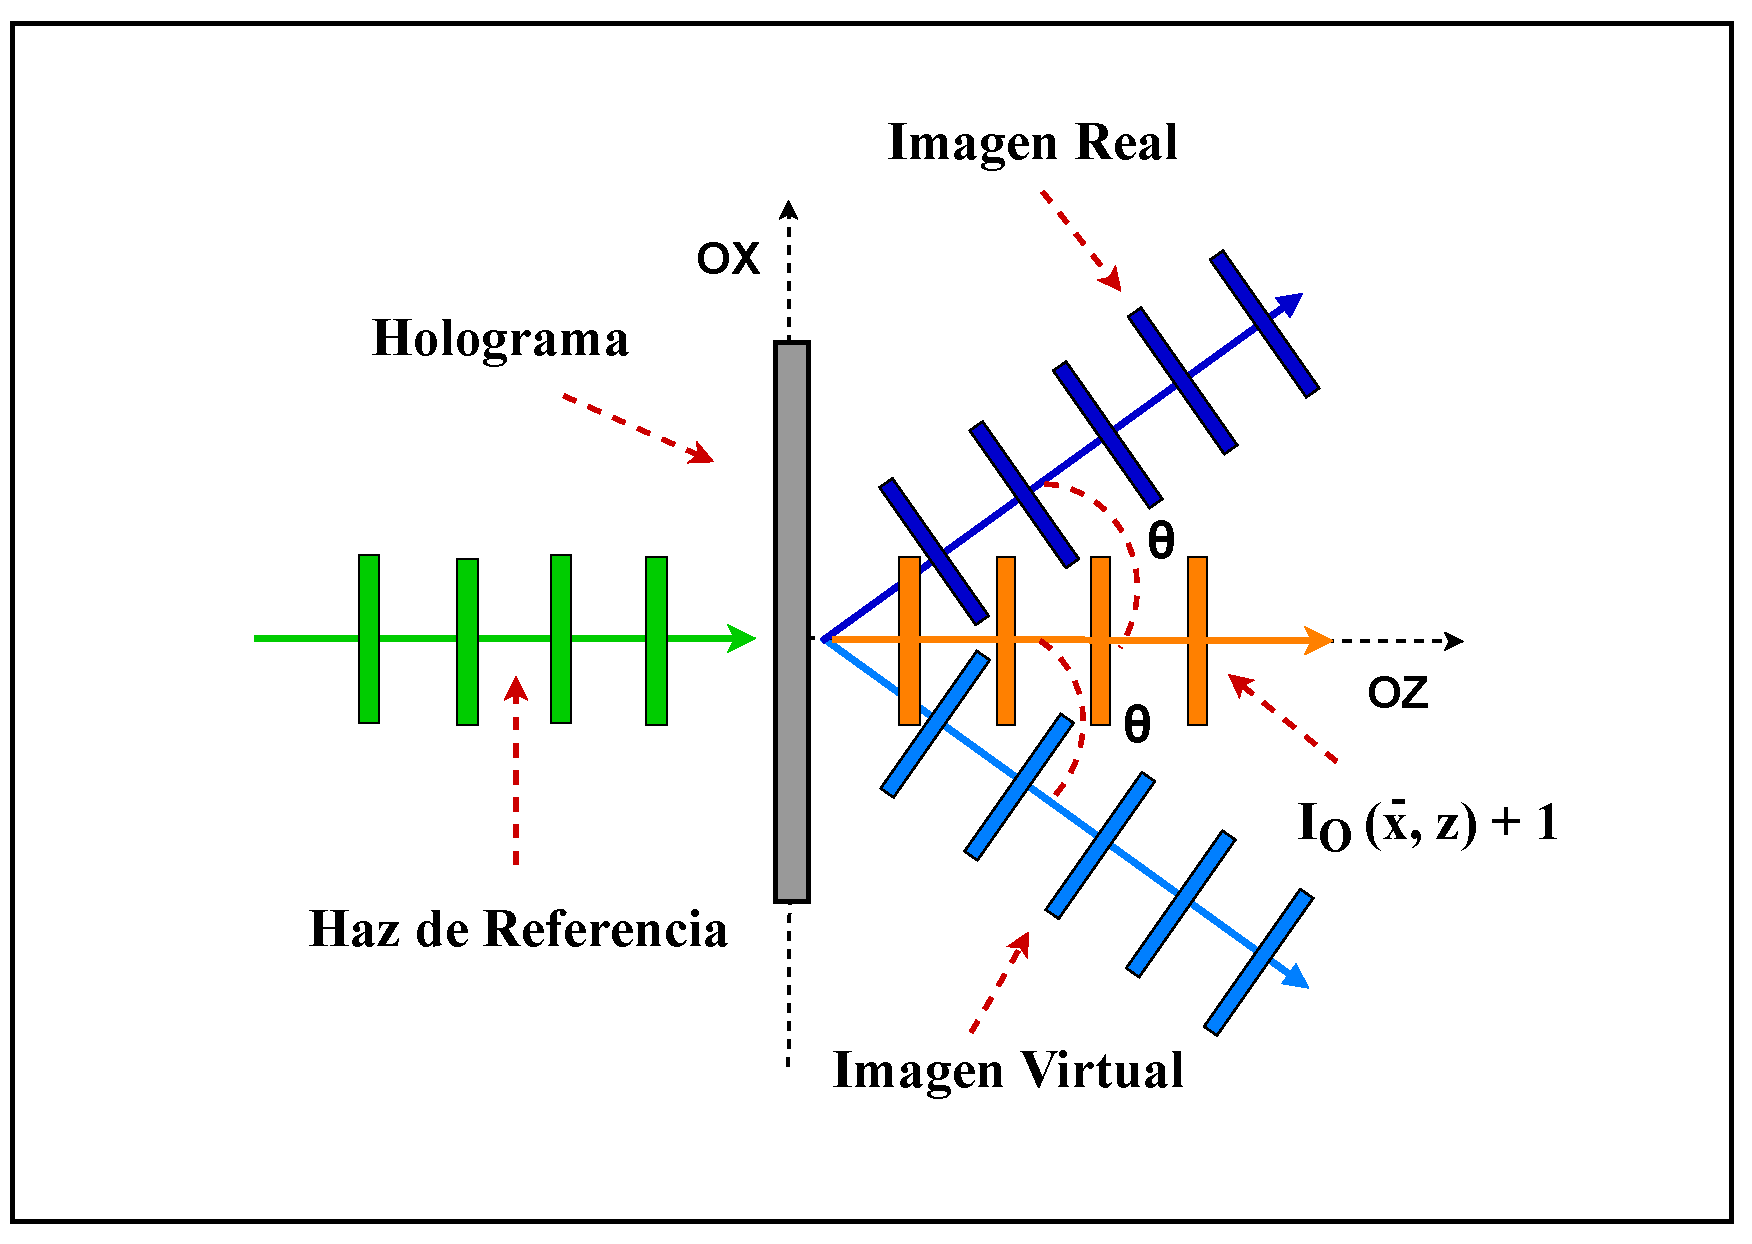
\includegraphics[scale = 0.4]{figure_3.pdf}
    \caption{Etapa de reconstrucción para una configuración fuera de eje.}
    \label{figura3}
\end{figure}
%%%
Consecuentemente,
%%%
\begin{figure}[b!]
    \centering
    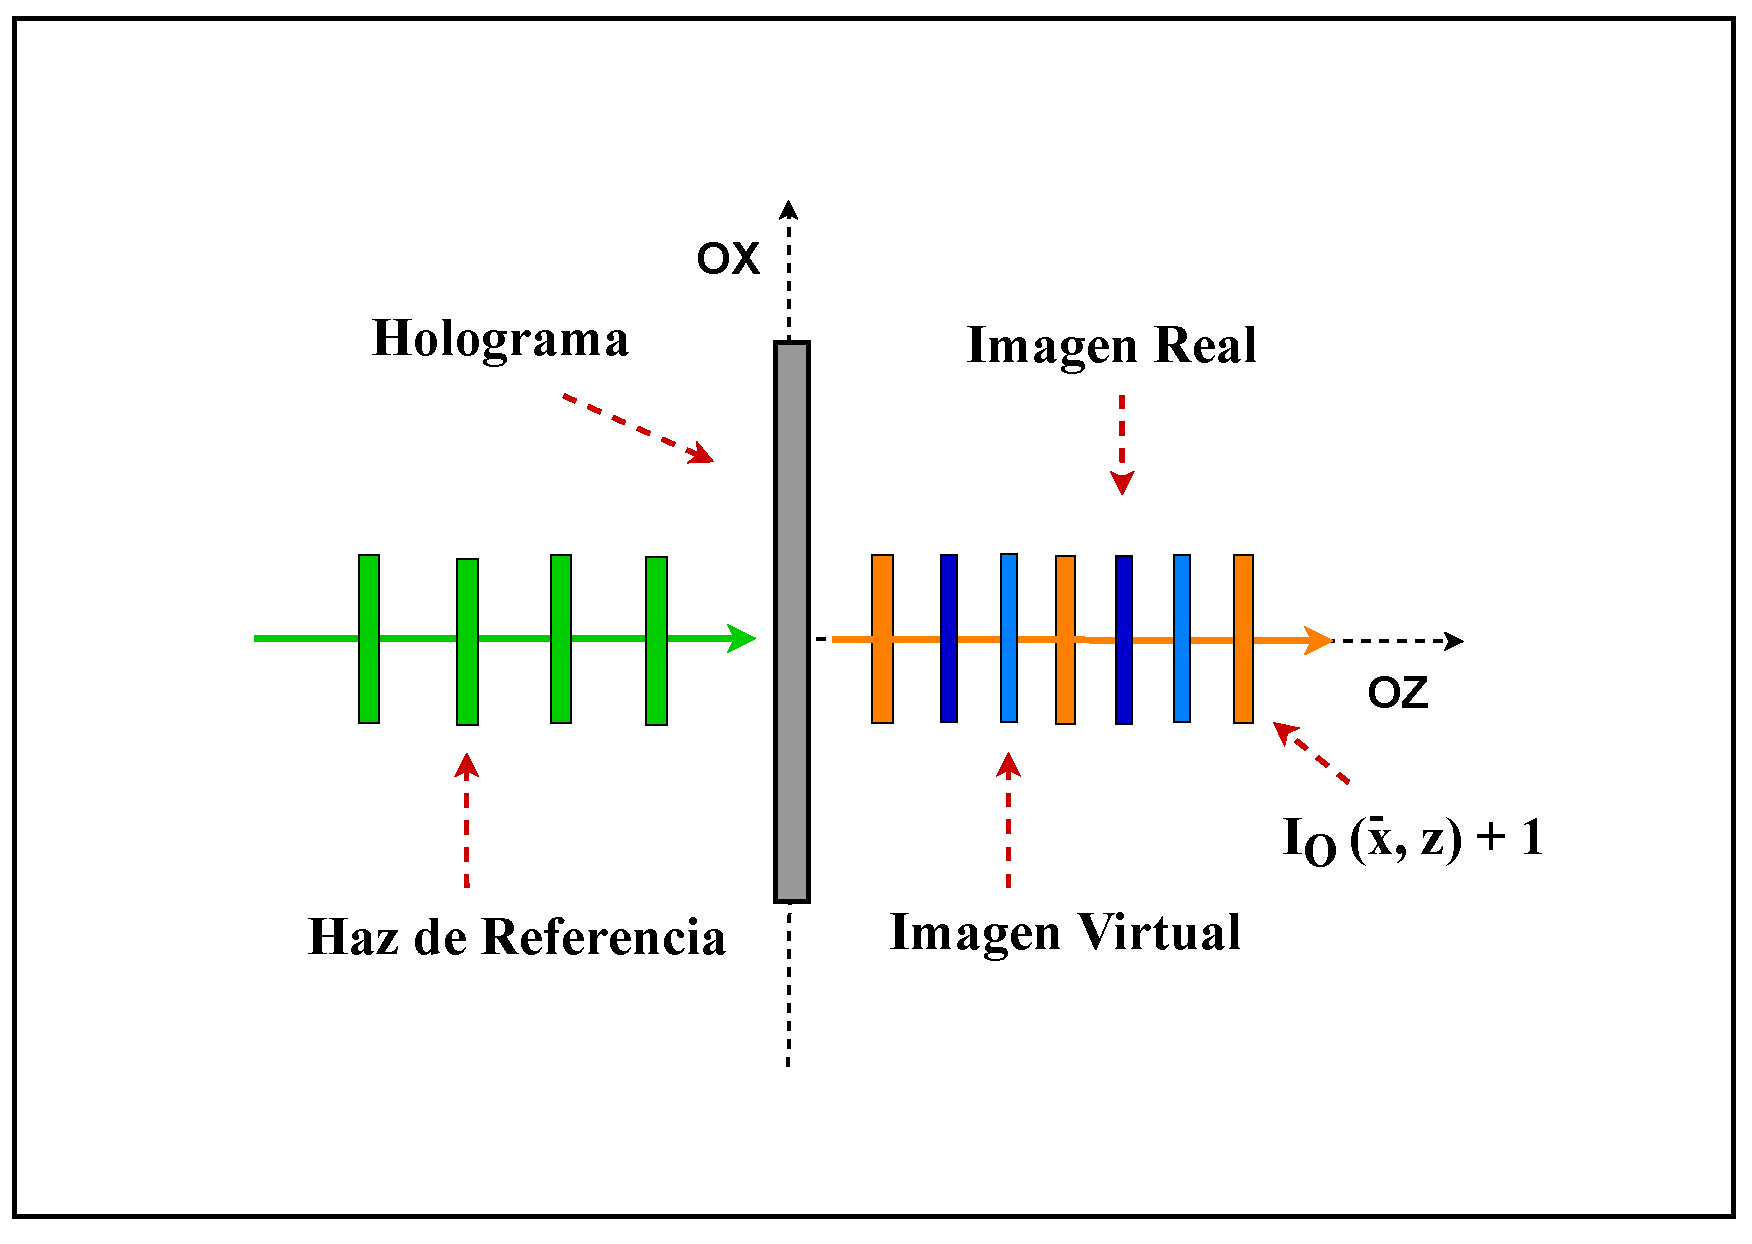
\includegraphics[scale = 0.4]{figure_4.pdf}
    \caption{Etapa de reconstrucción para una configuración en eje.}
    \label{figura4}
\end{figure}
%%%
las componentes reconstruidas se difractarán en la misma dirección sobre el eje óptico $OZ$.  \\ \\
%%%
Esquematizamos la etapa de reconstrucción para montajes tipo en eje en la Fig.\ref{figura4}. Al igual que antes, el haz naranja representa la propagación de la componente $I_O (\Vec{x}, z) +  1 $ de la Ec.(\ref{Ec.10}), mientras que los haces azules corresponden a la propagación de las ondas asociadas a la reconstrucción de la imagen real y a la imagen virtual del objeto. Por lo tanto, dada la existencia de un solapamiento en la propagación de los tres haces, finalmente  el observador visualizará una imagen borrosa cuando $\theta \sim 0$. \\ \\
%%%
A pesar de que la técnica holográfica es un buen mecanismo  de formación de imágenes,  finalmente la holografía clásica recrea tanto la imagen del objeto como  las otras componentes que forman el patrón de intensidad. Por lo tanto, la visualización de la imagen se ve limitada tanto  por  la reconstrucción de las intensidades  sin modular del haz objeto y del haz de referencia, como por el efecto de la imagen gemela. Además, la calidad de imagen dependerá de si se trata de una configuración fuera de eje o en eje, ya que la reconstrucción de las componentes que forman el patrón de intensidad se solapan entre sí para ángulos significativamente pequeños. \\ \\
%%%
Podemos concluir que  el concepto de holografía es la combinación  del principio de interferencias y del modelo de propagación en el espacio libre asociado a difracción de las distribuciones de amplitud del campo electromagnético. Como ya hemos visto, ambos conceptos son necesarios para desarrollar tanto la etapa de registro como la etapa de reconstrucción. Por un lado, el principio de  interferencias permite codificar la información sobre el contorno y  la profundidad de la imagen del objeto a partir de hacer interferir dos haces entre sí. Por otro lado,  la difracción   permite  descodificar dicha información y trasladarla desde un plano transversal $XY$ a otro cualquiera. El mecanismo de la holografía consiste por tanto, en redirigir los haces correspondientes a cada punto del objeto a otro punto concreto. Por ese motivo, tras conseguir aislar la forma del campo luminoso emergente de un objeto, podemos recrear su imagen en cualquier otro punto aunque el objeto no éste presencialmente en el sistema. \\ \\
%%%
Con el fin de recrear una imagen nítida y clara del objeto para todos los tipos de configuración, la holografía clásica se complementa con las técnicas digitales más actuales.
%%%%%%%%%%%%%%%%%%%%%%%%%%%%%%
%%% HOLOGRAFÍA DIGITAL
%%%%%%%%%%%%%%%%%%%%%%%%%%%%%%
\section{Holografía digital}
La holografía digital es una técnica  de formación de imágenes que usa elementos digitales en el proceso, los cuales permiten aplicar métodos  computacionales sobre el concepto clásico de la holografía \cite{9}. Nace ante la necesidad de solucionar la limitación de la técnica convencional para ciertos montajes, de modo que permite recrear la imagen del objeto con claridad en todos los tipos de configuración.  Aunque la base de la técnica es la misma que en la holografía clásica, se diferencia en el uso de un dispositivo digital  para registrar numéricamente la intensidad resultante de la interacción entre el haz objeto y el haz de referencia.  Además, la tecnología actual permite aplicar cálculos digitales sobre los datos recogidos en el registro, manipular la información computacionalmente para buscar las frecuencias espaciales deseadas, propagar la distribución de amplitud del campo para llevar a cabo un reenfoque digital, tomar medidas cuantitativas del objeto y  simular tanto la etapa de registro como la etapa de reconstrucción  en el ordenador. En este último caso, el objeto no existirá físicamente por lo que se debe simular la etapa de registro con un objeto sintético\footnote{Un objeto sintético es  aquel  que se crea digitalmente de forma que reproduce las propiedades y las dimensiones de uno real.}. \\ \\  
%%% 
Un holograma digital\footnote{En adelante, se hace referencia  al holograma digital como holograma, mientras que se hace referencia al holograma convencional de la holografía clásica como holograma analógico.} es el registro electrónico del patrón de intensidad de una interferencia cuya señal  puede ser procesada y/o trasmitida   a la transmitancia en amplitud $t (\Vec{x})$ de un modulador espacial de luz, como puede ser una pantalla de cristal líquido. La monitorización de esta intensidad facilita la descodificación de la estructura tridimensional del objeto dado que permite aplicar métodos numéricos complejos en el análisis de la transmitancia $t (\Vec{x})$. \\ \\ 
%%%
Al igual que en la holografía clásica, el mecanismo de la holografía digital consta  de dos partes diferenciadas. En la etapa de registro, se almacena  la intensidad de la interferencia entre el frente de ondas objeto y el frente de ondas de referencia mediante el uso de un sensor electrónico pixelado\footnote{Un sensor electrónico pixelado es un elemento óptico que forma parte de una cámara digital. Dicho sensor es una matriz compuesta por elementos fotosensibles que convierte la luz recibida en señales eléctricas, las cuales pueden ser transformadas, manipuladas, analizadas y representadas como un patrón.}, mientras que en la etapa de reconstrucción, se reconstruye  la distribución de amplitud emergente del objeto a partir de manipular y reproducir la información del registro electrónico previo.  Los procesos necesarios para descodificar dicha información dependerán de si existe o no un solapamiento en el dominio de frecuencias espaciales de los haces mezclados en el registro.  Por un lado, se expondrá la técnica de filtrado  \cite{10} como un método típicamente utilizado  para reconstruir el frente de ondas objeto cuando el  ángulo interferencial es lo suficientemente grande para no solapar los haces entre sí. Por otro lado, se presentará el método de variación de fase \cite{11} como  alternativa a la técnica de filtrado, es decir, cuando los haces se solapen en el dominio de Fourier.\\\\
%%%
La técnica de filtrado es un método que permite   recrear la imagen tridimensional de un objeto sin reconstruir las contribuciones del holograma que puedan entorpecer la observación de su imagen. Esta técnica consiste en transformar la irradiancia espacial al dominio de frecuencias espaciales con el fin de separar las componentes que forman el patrón de intensidad en términos disjuntos. Una vez se separan las componentes entre sí, se aplica un filtro pasabanda de frecuencias espaciales para extraer el término deseado por lo que, tras aplicar el filtro, las componentes restantes quedan suprimidas del sistema. Así, se  consigue  recrear  una única imagen del objeto y por consiguiente, se elimina el efecto visual de la imagen gemela y del halo.\\ \\
%%%
En la etapa de registro  de la técnica de filtrado, sustituimos el holograma analógico de la Fig.\ref{figura1}, o  de la Fig.\ref{figura2},  por un sensor pixelado de una cámara electrónica conectada directamente al ordenador. Así, la interferencia entre ambos frentes de onda ocurre sobre este sensor  en el plano del holograma,  por lo que si suponemos que la cámara esta formada por un sensor ideal que no pierde información en el procesado de la señal, lograremos registrar la intensidad de la interferencia $I(\Vec{x},z)$ sin pérdidas. \\ \\
%%%
En la etapa de reconstrucción, comenzamos analizando espectralmente el patrón de intensidad de la Ec.(\ref{Ec.7}). Para ello,  aplicamos la transformada de Fourier\footnote{La transformada de Fourier bidimensional de una función $f(\Vec{x})$, se define  como  $\Tilde{f}(\Vec{u}) = \Tilde{f}(u_x,u_y) = \int \int f(\Vec{x}) e^{-i 2 \pi \Vec{u} \Vec{x}}d^2\Vec{x}$. Su aplicación sobre $f (\vec{x})$ se denota como $\mathscr{F} \{ f (\vec x); \vec{u} \}$, mientras que se asigna el símbolo $\sim$  a la función  resultante.} sobre cada uno de los términos que la constituyen, de manera que obtenemos
%%%
\begin{equation}
    \mathscr{F}\{\mid A_O (\vec{x}, z) \mid ^{2}; \vec{u}\} + \mathscr{F}\{1; \Vec{u}\} = \tilde{A}_O(\Vec{u},z) \circledast \tilde{A}_O^{*} (-\Vec{u},z)  + \delta(\Vec{u})= \tilde{A}_O(\Vec{u},z) \otimes \tilde{A}_O (\Vec{u},z) + \delta(\Vec{u}).
    \label{Ec.11}
\end{equation}
%%%
\begin{equation}
    \mathscr{F}\{A_O (\Vec{x}, z) e^{i k x \sin{\theta}}; \vec{u} \} = \tilde{A}_O(\Vec{u}, z) \circledast \delta(u_x -\frac{\sin{\theta}}{\lambda}, u_y).
\label{Ec.12}
\end{equation}
%%%
\begin{equation}
    \mathscr{F}\{A_O^{*} (\Vec{x}, z) e^{-i k x \sin{\theta}}; \vec{u} \}  = \tilde{A}^{*}_O(\Vec{u}, z) \circledast \delta(u_x + \frac{\sin{\theta}}{\lambda}, u_y).
\label{Ec.13}
\end{equation}
%%%
Por simplicidad,   hemos ignorado los factores que dependen únicamente de $z$ dado que son constantes  en el plano de registro y no afectan al razonamiento posterior. Cabe destacar que hemos denotado con el símbolo $\otimes$  a la operación de correlación y que, en la Ec.(\ref{Ec.11}), hemos utilizado la relación que existe entre las operaciones de correlación y convolución\footnote{Se expone la relación entre la convolución, la correlación y las transformadas de Fourier en \cite{12}.}. Como indica la Ec.(\ref{Ec.11}), la transformada de Fourier de la intensidad de la onda objeto en el plano del holograma es la autocorrelación del espectro de frecuencias de la distribución de amplitud del objeto.  Por otro lado, el factor $\delta(\vec{u}) = \delta(u_x,u_y)$ corresponde a  una delta de Dirac centrada en el origen de frecuencias espaciales, mientras que   el factor $ \delta(u_{x} \mp \frac{\sin{\theta}}{\lambda}, u_y)$,  es una delta de Dirac desplazada una distancia $\pm \sin{\theta}/\lambda$  en $u_x$ respecto al origen. \\ \\
%%%
De esta manera,  el espectro de la irradiancia es una composición de las transformadas de Fourier de las Ecs.(\ref{Ec.11})-(\ref{Ec.13}), por lo que la intensidad en el espacio de Fourier es
%%%
\begin{align}
     \tilde{I}(\Vec{u},z) &=  \Tilde{DC}(\Vec{u},z) + \tilde{A}_O(\Vec{u}, z) \circledast \delta(u_x - \frac{\sin{\theta}}{\lambda}, u_y) + \tilde{A}^{*}_O(\Vec{u}, z) \circledast \delta(u_x +\frac{\sin{\theta}}{\lambda}, u_y),
     \label{Ec.14}
\end{align}
%%%
siendo  $\tilde{DC}( \Vec{u}, z) = \Tilde{A}_O (\Vec{u},z) \otimes \tilde{A}_O (\Vec{u},z) + \delta(\Vec{u})$. La convolución  en la Ec.(\ref{Ec.14}) entre la transformada de Fourier de la onda objeto  y el factor $ \delta(u_{x} \mp \frac{\sin{\theta}}{\lambda}, u_y)$ es una versión de esta función centrada en una posición $(\pm \frac{\sin{\theta}}{\lambda}, 0)$, de modo que 
%%%
\begin{align}
     \tilde{A}_O(\Vec{u}, z) \circledast \delta(u_x - \frac{\sin{\theta}}{\lambda}, u_y) &= \tilde{A}_O (u_x - \frac{\sin{\theta}}{\lambda}, u_y,z), \nonumber \\
      \tilde{A}^{*}_O(\Vec{u}, z) \circledast \delta(u_x + \frac{\sin{\theta}}{\lambda}, u_y) &= \tilde{A}^{*}_O (u_x +\frac{\sin{\theta}}{\lambda}, u_y,z).
     \label{Ec.15}
\end{align}
%%%
Identificamos por tanto, tres términos independientes y separados frecuencialmente entre sí, por lo que el espectro frecuencial de la intensidad viene dada por 
%%
\begin{equation}
     \Tilde{I}(\vec{u}, z) = \tilde{DC}( \Vec{u}, z) + \tilde{A}_O (u_x -\frac{\sin{\theta}}{\lambda}, u_y,z) + \tilde{A}_O^{*} (u_x +\frac{\sin{\theta}}{\lambda}, u_y,z).
     \label{Ec.16}
\end{equation}
%%%
El primer término corresponde a la transformada de Fourier de la suma de las intensidades  de la onda objeto y de la onda de referencia en el plano del holograma. Al localizarse en torno al origen de frecuencias lo identificamos como el orden cero de difracción. La segunda componente describe el espectro de Fourier de la onda  objeto en el plano del holograma desplazado una distancia $\sin{\theta} /\lambda$ en la coordenada $u_x$ respecto al origen de frecuencias espaciales. A su vez, identificamos la tercera componente como el espectro de Fourier de la onda objeto complejo conjugada en una posición $- \sin{\theta} /\lambda$ del origen. Por lo tanto, al igual que en la holografía clásica,   los dos últimos términos corresponden a la reconstrucción de la imagen real y de la imagen virtual del objeto, respectivamente. Como ambas imágenes se encuentran desviadas simétricamente alrededor de  $\Tilde{DC}(\Vec{u},z)$, las identificamos  como el primer orden de difracción y, para diferenciarlas, asignamos el orden $+1$ de difracción a la segunda componente y el orden $-1$ a la tercera. Ahora, vamos a considerar que estos tres órdenes de difracción tienen extensiones finitas en el dominio de Fourier\footnote{Esta restricción se cumple en la práctica dado que todo sistema real de formación de imágenes transmite una banda  de frecuencias limitada en el dominio de Fourier \cite{13}.}.  Es sencillo probar que la extensión de la banda de frecuencias del patrón de difracción del objeto $A_O (\Vec{x},z)$ se mantiene para cualquier  $z$ dado que la función de transferencia para la propagación libre sólo modifica la fase de las diferentes frecuencias espaciales. Por ello,  si consideramos que el objeto tiene la banda frecuencial limitada y centrada alrededor de $\Vec{u} = 0$ que se extiende simétricamente con un tamaño $\Delta$ en la dirección $u_x$, podemos suponer que la banda del patrón de difracción de $\tilde{A}_O (u_x - \frac{\sin{\theta}}{\lambda}, u_y,z)$ y $\tilde{A}_O^{*} (u_x +\frac{\sin{\theta}}{\lambda}, u_y,z)$ se extenderá simétricamente con la misma extensión. Dado que el orden $0$ de difracción es básicamente la autocorrelación de $\tilde{A_O} (\Vec{u},z)$ en el dominio de frecuencias espaciales, su banda tendrá una extensión doble que la de los órdenes $\pm 1$.\\ \\
%%%
En la Fig.\ref{figura5}, esquematizamos los tres términos que constituyen la intensidad de la Ec.(\ref{Ec.16}). Por un lado, en el centro del sistema bidimensional de frecuencias espaciales, representamos el orden $0$ de difracción como un círculo de color naranja. Por otro lado, representamos los órdenes $\pm 1$ de difracción  como  dos círculos azules  desplazados, respectivamente, una distancia $\pm \sin{\theta}/\lambda$ en  $u_x$  del orden $0$ de difracción, por lo que están simétricamente posicionados respecto al origen del sistema. Como ya sabemos, el orden $0$ esta formado por la autocorrelación de la  transformada de Fourier de la  distribución de amplitud del haz objeto en el plano del holograma, por lo que el tamaño de su banda espectral será dos veces mayor que el tamaño  de las bandas de los órdenes $\pm 1$ individualmente. Por ese motivo,  representamos al círculo naranja  con un radio dos veces  mayor que los círculos de color azul. Cabe destacar que, en el esquema,  hacemos referencia al tamaño de la banda  del objeto como $\Delta$ y al tamaño del orden $0$ de difracción como $2\Delta$. De acuerdo con la Fig.\ref{figura5}, siempre que 
%%%
\begin{figure}[b!]
    \centering
    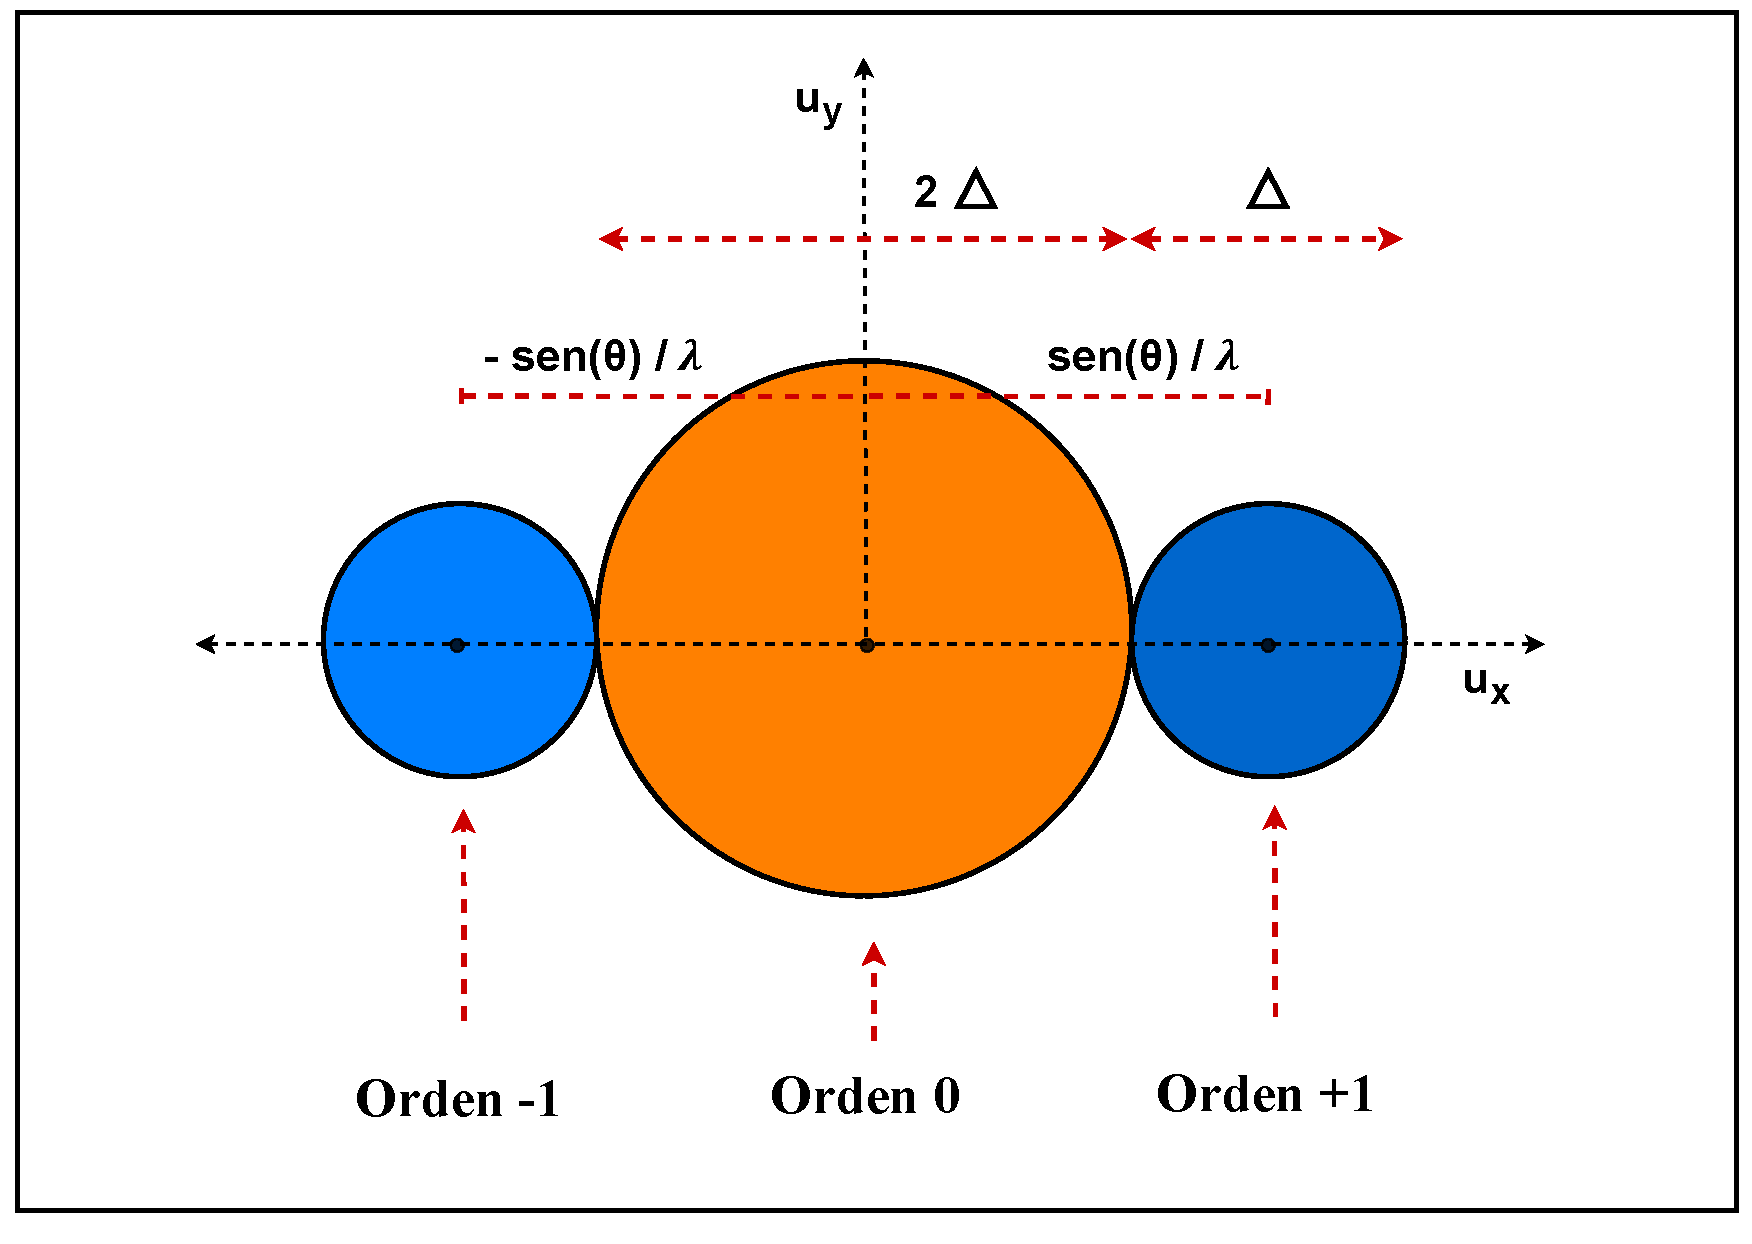
\includegraphics[scale = 0.4]{figure_5.pdf}\\
    \caption{Esquema del espectro de Fourier de la irradiancia del holograma.}
    \label{figura5} 
\end{figure}
%%%
\begin{equation}
    \frac{3 \Delta}{2} \leq \frac{\sin{\theta}}{\lambda},
    \label{Ec.17}
\end{equation}
%%
el contenido frecuencial de cada orden quedará separado entre sí. Por lo tanto, la banda de frecuencias del patrón de difracción del objeto en el plano del holograma no solapará con el resto de las bandas. Esta condición es un requisito necesario para que este método nos proporcione una reconstrucción fidedigna del objeto original, de modo que si se cumple la condición de la Ec.(\ref{Ec.17}), se podrá llevar a cabo la técnica de filtrado como método de reconstrucción. \\\\
%%%
Si la Ec.(\ref{Ec.17}) se cumple, para  reconstruir la imagen real del objeto haciendo uso de la técnica de filtrado, bastará con aplicar un filtro pasabanda de frecuencias espaciales al holograma registrado que permita extraer exclusivamente el ancho de banda espectral del orden $+1$ de difracción correspondiente a la reconstrucción de la imagen real. Tras aplicarlo, obtenemos
%%%
\begin{equation}
    \Tilde{I}'(u_x - \frac{\sin{\theta}}{\lambda}, u_y, z) = \mathscr{H}_1 (\Vec{u}) \Tilde{I} (\Vec{u}, z) = \tilde{A}_O (u_x - \frac{\sin{\theta}}{\lambda}, u_y,z),
    \label{Ec.18}
\end{equation}
%%%
siendo $\mathscr{H}_1 (\Vec{u})$  la función de transferencia del filtro para el orden $+1$ de difracción  y  $\Tilde{I}'(u_x - \frac{\sin{\theta}}{\lambda}, u_y, z)$ la componente ya filtrada. \\ \\
%%%
Si a continuación, desplazamos el término filtrado de la Ec.(\ref{Ec.18}) desde la posición $ -\sin{\theta}/\lambda$  hasta el origen  de frecuencias espaciales y luego le aplicamos la transformada de Fourier inversa\footnote{La transformada de Fourier inversa de una función bidimensional $\Tilde{f}(\Vec{u})$, se define como $f (\Vec{x}) = f (x,y) = \int \int \tilde{f}(\Vec{u}) e^{ j 2 \pi\Vec{u} \vec{x}} d^{2}\Vec{u}$. Se hace referencia  a la aplicación de la transformada de Fourier inversa sobre $\tilde{f} (\Vec{u})$ como $\mathscr{F}^{-1} \{ \tilde{f} (\Vec{u}) ; \Vec{x}\}$.}, finalmente, conseguimos reconstruir la distribución de amplitud del haz objeto  en el plano del holograma como
%%%
\begin{equation}
    U (\Vec{x}, z) = \mathscr{F}^{-1}\{\Tilde{I}'(\Vec{u},z); \vec{x} \} = A_O (\vec{x}, z).
    \label{Ec.19}
\end{equation}
%%%
La distribución de amplitud de la Ec.(\ref{Ec.19}) es la onda objeto en el plano del holograma, por lo que hemos conseguido suprimir el resto de las componentes de la intensidad con la técnica de filtrado. Consecuentemente, hemos conseguido eliminar tanto el efecto  de la imagen gemela como la reconstrucción del halo de luz central. \\ \\
%%%
Dado que la distancia de separación entre las componentes depende directamente  del ángulo interferencial, si suponemos que el ángulo es considerablemente pequeño, las componentes que forman el patrón de intensidad no se desacoplarán, es decir, no se cumplirá la condición de la Ec.(\ref{Ec.17}).  Por lo tanto, en configuraciones con $\theta \sim 0$, los tres órdenes de difracción se solaparán entre sí, por lo que no lograremos extraer suficiente información del orden $+1$ de difracción. Tampoco podremos utilizar esta técnica si el ancho de banda espectral del objeto es muy grande dado que las componentes seguirán solapadas aún estando frecuencialmente separadas entre sí. Consecuentemente, no podremos formar una imagen fidedigna del objeto.\\ \\
%%%
Podemos concluir que la técnica de filtrado es un  método de formación de imágenes rápido y eficaz dado que nos pemite recrear la imagen tridimensional del objeto a partir de registrar una única captura de la irradiancia.  Sin embargo, su principal desventaja reside en que no puede llevarse a cabo cuando el ángulo de la interferencia entre haces es significativamente pequeño o cuando el ancho de banda espectral del objeto es muy grande, ya que las componentes no se desacoplarán completamente entre sí y por ende, perdemos información de la onda objeto en la reconstrucción de su imagen.\\ \\
%%%
Ante la necesidad de suprimir la reconstrucción de la imagen virtual y la intensidad luminosa del orden cero de difracción cuando la técnica de filtrado no lo permite, sin perder información en el proceso, nace una técnica alternativa conocida como el método de variación de fase \cite{11}. Esta técnica  consiste  en extraer la distribución de amplitud del campo emitido por el objeto, inicialmente desconocida, a partir de realizar tres capturas distintas del patrón de intensidad en el plano del holograma. Para llevar a cabo estas capturas, en la etapa de registro, se debe incorporar un modulador de fase que permita añadir una fase constante controlable al haz de referencia. De esta manera, se obtiene un sistema de tres ecuaciones formado por  tres  irradiancias. Si se resuelve este sistema de ecuaciones de forma que se consiga aislar la componente asociada  a la reconstrucción de la imagen real del objeto, se puede reconstruir dicha imagen sin el resto de las contribuciones. Por lo tanto, es una técnica que también elimina el efecto visual de la imagen gemela y el halo de luz central que se recrea junto a la imagen del objeto. \\ \\
%%%
El montaje de la etapa de registro para el método de variación de fase  es similar al expuesto en la Fig.\ref{figura2} pero añadiendo un modulador de fase en la trayectoria del haz de referencia, de modo que cuando se propaga a través de él, se añade una fase  constante $\phi_p$ a la propagación de dicho frente. Así, conseguimos registrar tres patrones de intensidad con una fase diferente en cada distribución de amplitud asociada al haz de referencia.\\\\
%%%
Por lo tanto, tras añadir el modulador de fase en el montaje, el patrón de intensidad en el plano de la interferencia es
%%%
\begin{equation}
   I_p (\Vec{x}, z) =  \mid  U_O (\Vec{x}, z) + U_R (\Vec{x}, z)e^{i \phi_p}\mid ^{ 2 },
    \label{Ec.20}
\end{equation}
%%%
donde el subíndice $p$ indica el número de la captura de la irradiancia.  \\ \\
%%%
Siguiendo los mismos pasos que nos llevaron a obtener la intensidad de la Ec.(\ref{Ec.7}) y omitiendo los factores constantes dependientes de $z$, la forma extendida de la Ec.(\ref{Ec.20}) se puede expresar como
%%%
\begin{equation}
   I_p (\Vec{x}, z) = DC (\Vec{x}, z) +  e^{-i \phi_p} A_O (\Vec{x}, z) e^{i k x \sin{\theta}}   + e^{i \phi_p}A_O ^{*}(\Vec{x}, z)e^{-i k x \sin{\theta}},
    \label{Ec.21}
\end{equation}
%%%
siendo $DC (\Vec{x}, z) = \mid A_O (\Vec{x}, z) \mid ^{2} + 1 $.\\\\
%%%
Por lo tanto,  el sistema de tres ecuaciones formado por tres irradiancias viene dado por
%%%
\begin{align}
    I_1 (\Vec{x}, z) = &  DC (\Vec{x}, z) + e^{-i \phi_1} A_O (\Vec{x}, z) e^{i k x \sin{\theta}} + e^{i \phi_1}A_O ^{*}(\Vec{x}, z) e^{-i k x \sin{\theta}} \nonumber \\
    I_2 (\Vec{x}, z) = &  DC (\Vec{x}, z) + e^{-i \phi_2} A_O (\Vec{x}, z) e^{i k x \sin{\theta}}  + e^{i \phi_2} A_O ^{*}(\Vec{x}, z) e^{-i k x \sin{\theta}}\nonumber \\
    I_3 (\Vec{x}, z) = &   DC (\Vec{x}, z) + e^{-i \phi_3}A_O (\Vec{x}, z) e^{i k x \sin{\theta}} + e^{i \phi_3} A_O ^{*}(\Vec{x}, z) e^{-i k x \sin{\theta}}.
    \label{Ec.22}
\end{align}
%%%
A continuación, debemos operar las irradiancias que componen la Ec.(\ref{Ec.22}) entre sí hasta conseguir  aislar la distribución de amplitud del  haz objeto $A_O (\Vec{x}, z) e^{i k x \sin{\theta}}$. La regla de Cramer nos proporciona la solución del sistema de ecuaciones como
%%%
\begin{equation}
    A_O (\Vec{x}, z) e^{i k x \sin{\theta}} = \frac{  
    \begin{vmatrix}
        1 & I_1(\Vec{x},z) & e^{i \phi_1}\\
        1 & I_2(\Vec{x},z) & e^{i \phi_2}\\
        1 & I_3(\Vec{x},z) & e^{i \phi_3}
    \end{vmatrix}
    }{D},
    \label{Ec.23}
\end{equation}
%%%
de modo que el sistema de ecuaciones lineales de la Ec.(\ref{Ec.23}) tendrá solución única siempre y cuando se satisfaga la condición
%%%
\begin{equation}
    D =   
    \begin{vmatrix}
        1 & e^{-i \phi_1} & e^{i \phi_1}\\
        1 & e^{-i \phi_2} & e^{i \phi_2}\\
        1 & e^{-i \phi_3}& e^{i \phi_3}
    \end{vmatrix}
    \neq 0.
    \label{Ec.24}
\end{equation}
%%%
Una elección usual para los tres valores de la fase constante es: $\phi_1 = 0$,  $\phi_2 = \frac{\pi}{2}$ y  $\phi_3 = \pi$. Con estos valores para los que, claro está, se cumple la condición de la Ec.(\ref{Ec.24}), obtenemos, a partir de la Ec.(\ref{Ec.23}), la distribución de amplitud del objeto en el plano del holograma como
%%%
\begin{equation}
   A_O (\vec{x}, z)e^{i k \sin{\theta}} = \frac{(1+i) I_1 (\Vec{x},z) - 2 I_2 (\Vec{x},z) + (1-i) I_3(\Vec{x},z)}{4i}.
    \label{Ec.25}
\end{equation}
%%%
Por lo tanto, podemos concluir que la distribución de amplitud de la Ec.(\ref{Ec.25}) corresponde a la onda objeto en el plano del holograma, por lo que conseguimos reconstruir  la imagen real del objeto sin recrear el resto de las componentes junto a ella. Por consiguiente, con este método, conseguimos eliminar  el efecto de la imagen gemela  y el halo de luz central recreado junto a las imágenes. \\ \\
%%%
El método de variación de fase de la holografía digital es  por tanto, una técnica  de formación de imágenes tridimensionales que  da solución al problema del solapamiento de las configuraciones en eje.  Su mayor ventaja es que no requiere de análisis numéricos complicados y que elimina la reconstrucción de las constribuciones que dificultan la visualización de la imagen  sin perder información en el proceso, de modo  que elimina el orden  $0$ y $-1$ de la reconstrucción. Por el contrario, su mayor desventaja reside en su falta de rápidez debido a que, en el método de variación de fase, la etapa de registro se debe de repetir un mínimo de tres veces para que el sistema de ecuaciones se pueda resolver. Además, cabe destacar que este método se utiliza únicamente cuando las componentes del espectro frecuencial de la intensidad no cumplen la Ec.(\ref{Ec.17}) y por ende, las bandas de frecuencias se superponen entre sí. Dicho de otro modo, su uso está limitado a interferencias con   $\theta \sim 0$ o en configuraciones en las que la  banda espectral del objeto sea muy grande.\\ \\
%%%
Hasta ahora, hemos reconstruido la onda objeto en el plano del holograma. Para recrear la distribución de amplitud emergente del objeto sobre el plano del objeto, debemos llevar a cabo un reenfoque de la  onda, es decir, debemos propagarla desde el plano del holograma hasta el propio plano sobre el que se encuentra el objeto. Este reenfoque se puede llevar a cabo de forma óptica o digital.\\\\
%%%
Por un lado, si queremos  recrear ópticamente la imagen del objeto, debemos transferir la información de la onda objeto de la Ec.(\ref{Ec.19}) o de la Ec.(\ref{Ec.25}) a la trasmitancia  $t(\Vec{x})$ de un modulador espacial de luz. Si a continuación, provocamos la incidencia normal del  haz de referencia sobre la transmitancia $t(\Vec{x})$, emergerá del modulador un frente de ondas que reproducirá la amplitud y la fase de la onda objeto a lo largo de su propagación. Dicho de otro modo, la amplitud y la fase de la onda objeto se replicará en cada uno de los planos transversales al eje óptico sobre el que se difracta, por lo que el observador podrá visualizar todo el campo tridimensional difractado por el objeto. \\ \\
%%%
Por otro lado, si queremos llevar a cabo un reenfoque digital de la onda objeto, debemos realizar la convolución entre la onda objeto en el plano del holograma y la respuesta impulsional conjugada de la propagación libre correspondiente a la distancia $z$ desde el objeto hasta el sensor. De esta manera, conseguimos difractar la onda hasta el plano donde se encuentra el objeto y, una vez la describimos  sobre él, representamos la imagen del objeto en el ordenador.  Por lo tanto, si propagamos la Ec.(\ref{Ec.19}) o  la Ec.(\ref{Ec.25}) hasta el plano objeto,  la distribución de amplitud emergente del objeto viene dada por
%%%
\begin{equation}
   U (\vec{x}, 0) = U (\vec{x}, z) \circledast h^{*} (\Vec{x}, z),
    \label{Ec.26}
\end{equation}
%%%
siendo   $h^{*} (\Vec{x}, z) =  e^{- i \frac{\pi {\mid \vec{x} \mid}^{2}}{z \lambda}}$ la respuesta impulsional conjugada.\\ \\
%%%
A continuación, con el fin de verificar el método de variación de fase en configuraciones en eje, simularemos computacionalmente las etapas de la holografía hasta reconstruir la distribución de amplitud compleja de un objeto sintético.
%%%%%%%%%%%%%%%%%%%%%%%%%%%%%%
%%% SIMULATION 
%%%%%%%%%%%%%%%%%%%%%%%%%%%%%%
\section{Verificación de la técnica}
Se puede comprobar la solidez del modelo teórico del método de variación de fase para montajes en eje a partir de simular los pasos que nos llevaron a obtener las Ecs.(\ref{Ec.25}) y (\ref{Ec.26}). Como ya sabemos, a diferencia de la fotografía que nos permite extraer únicamente la  amplitud de la distribución de amplitud compleja emergente de un objeto, el mecanismo de la holografía nos permite obtener su amplitud y su fase. Por ese motivo,  particularizaremos para  una onda objeto con distribución de amplitud compleja pura de fase, de modo que si  conseguimos reconstruir fielmente la fase del objeto original, demostraremos  la eficacia del método de variación de fase. \\ \\
El diagrama de flujo de la Fig.\ref{figura6} expone las pautas que deben seguirse para verificar dicha técnica en el ordenador.
%%%
\begin{figure}[tbh!]
    \centering
    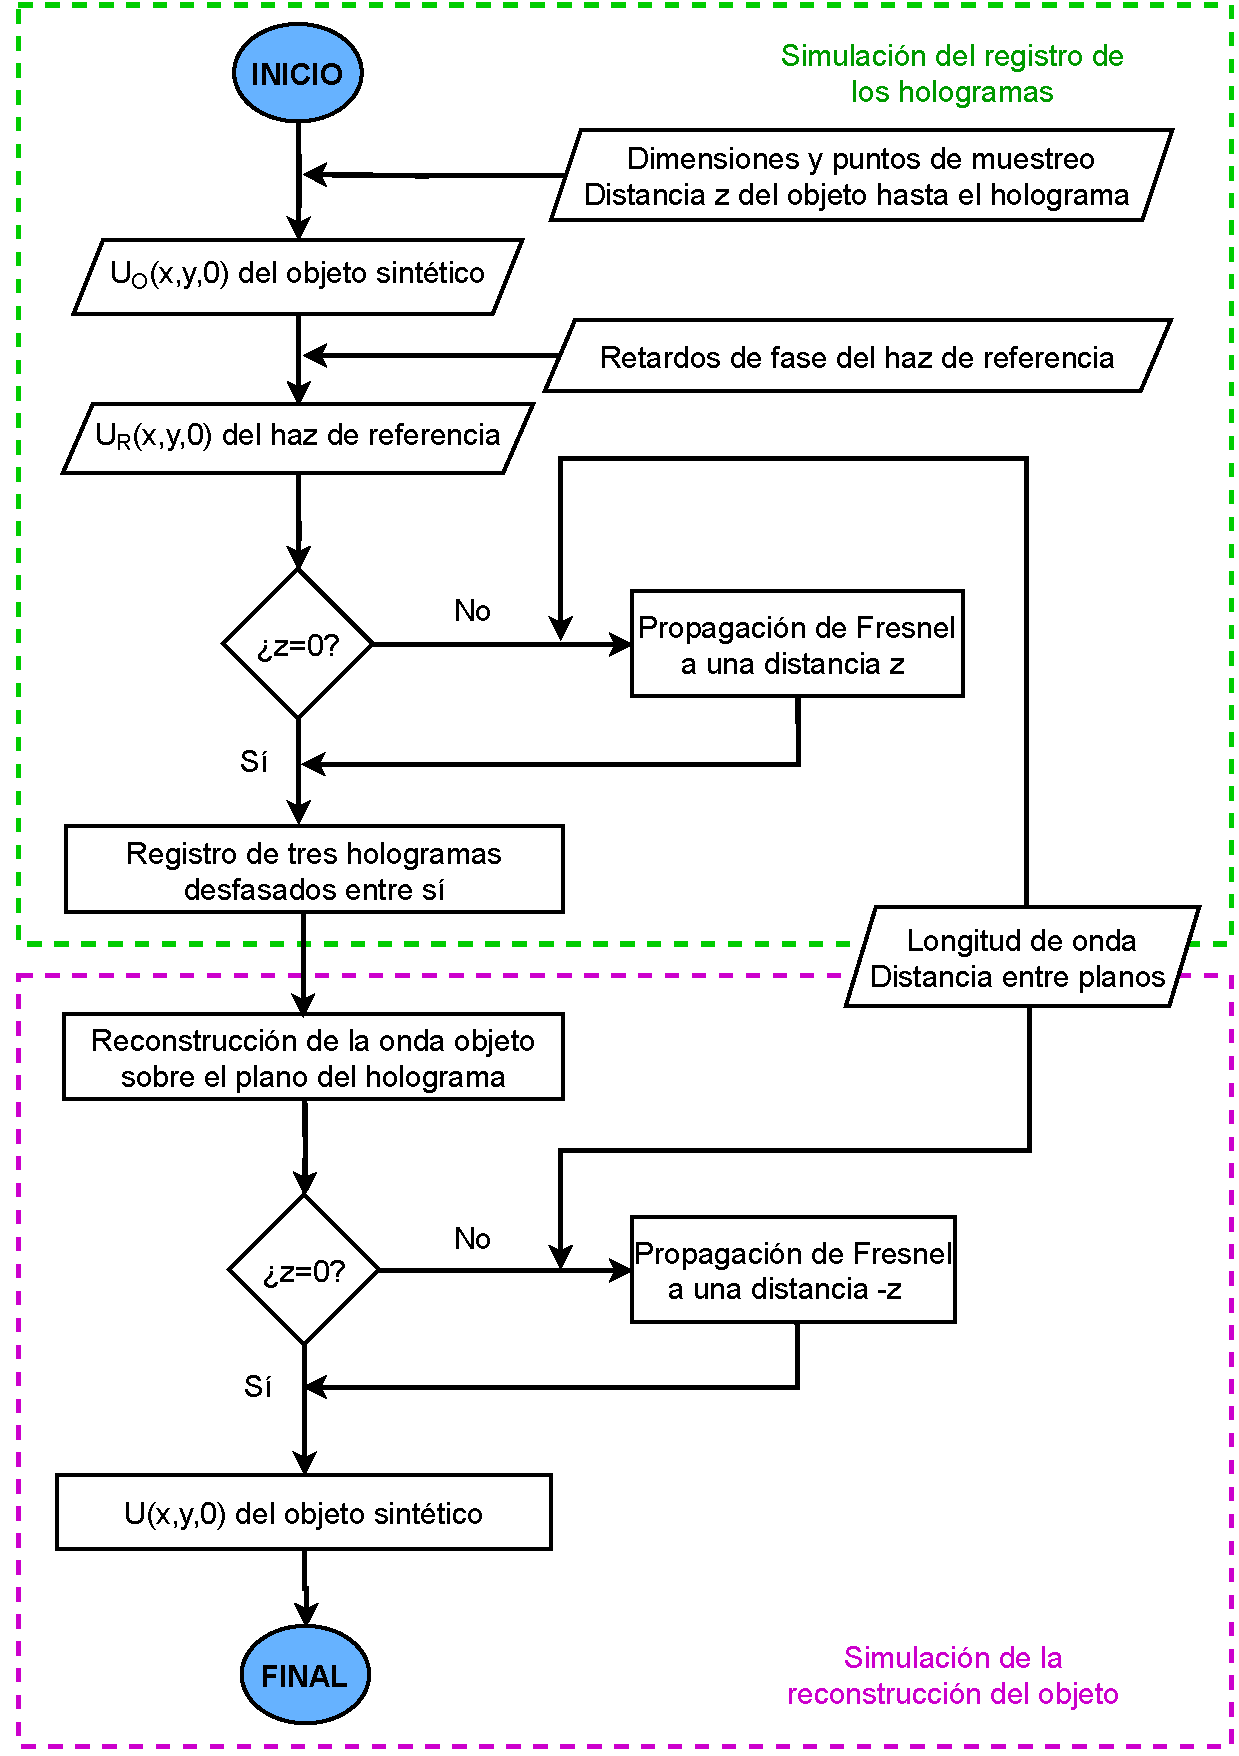
\includegraphics[scale = 0.55]{figure_6.pdf}
    \caption{Diagrama de flujo para simular el método de variación de fase.}
    \label{figura6}
\end{figure}
%%%
Además, cabe destacar que para simular el modelo teórico  se ha hecho uso de Python 3.9, ya que es una de las plataformas digitales más utilizadas para simular el mecanismo de la holografía dado que es un lenguaje completo de código abierto\footnote{Se puede acceder al código fuente que he desarrollado para verificar la válidez de la técnica en \textcolor{blue}{\url{https://www.dropbox.com/s/44kot4h21nzz1p7/VictoriaGomezBifante-AnexoTFG.pdf?dl=0}}.}.  \\ \\ 
%%%
En primer lugar, supongamos que la fase de la distribución de amplitud compleja de  la onda objeto, en el propio plano sobre el que se encuentra, es un disco de radio  $r_{max}$ de fase constante $\pi /2$ sobre un fondo uniforme de fase $0$ y que, además, dicho plano corresposponde al plano del holograma. A continuación, damos un valor fijo a la $\lambda$ de la fuente $\mathbb{F}$ de $500$ nm. Después, definimos los puntos de muestreo $N$  en la coordenada horizontal y en la coordenada vertical, respectivamente,  y creamos las gradillas bidimensionales  $N \times N$ a partir de ambas coordenadas. Estas gradillas describen el plano bidimensional $XY$  sobre el que se encuentra el objeto, por lo que si consideramos que el objeto se encuentra en $z = 0$ sobre el eje óptico $OZ$, el plano del holograma estará también sobre $z=0$. De modo que si particularizamos para $N = 550$ puntos de muestreo, tanto el plano del holograma como el plano del objeto estarán descritos por $550 \times 550$ puntos. \\ 
%%%
El método de variación de fase necesita registrar un mínimo de tres intensidades diferentes  de la interferencia entre la onda objeto con el haz de referencia cuando $\theta = 0$. Por ello, consideraremos que la distribución de amplitud de la onda de referencia es constante  y  le añadiremos una fase constante $\phi_{p}$ en cada registro de la  interferencia.
%%%
\begin{figure}[tb!]
\centering
    \begin{subfigure}[b]{0.45\textwidth}
        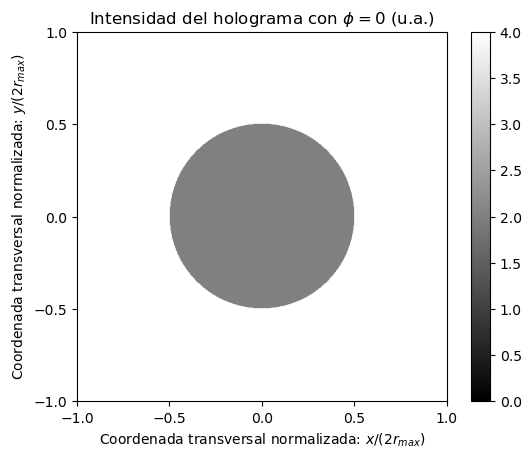
\includegraphics[width=1\textwidth]{figure_7.png}
        \caption{}
        \label{f7a}
    \end{subfigure}
    \begin{subfigure}[b]{0.45\textwidth}
        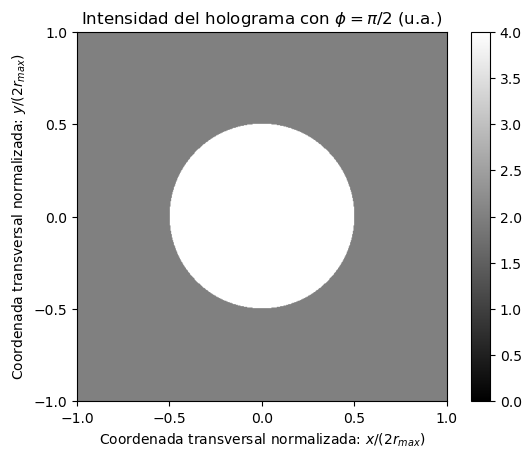
\includegraphics[width=1\textwidth]{figure_8.png}
        \caption{}
        \label{f7b}
    \end{subfigure}
    \begin{subfigure}[b]{0.45\textwidth}
        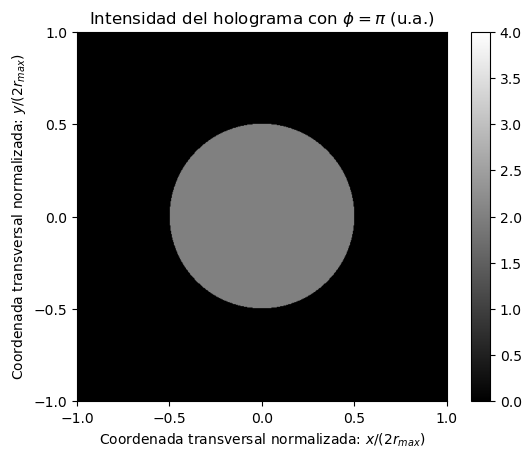
\includegraphics[width=1\textwidth]{figure_9.png}
        \caption{}
        \label{f7c}
    \end{subfigure}
    \begin{subfigure}[b]{0.45\textwidth}
        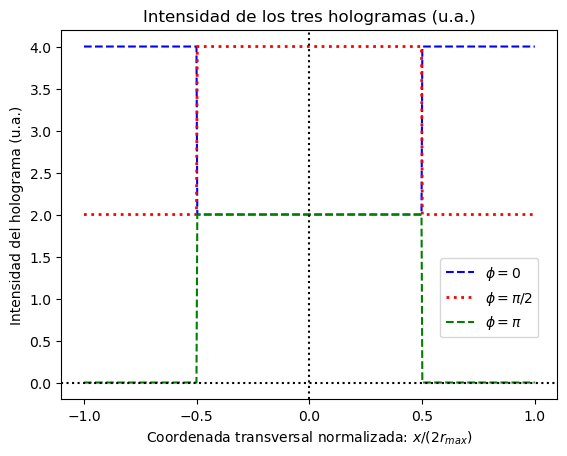
\includegraphics[width=1\textwidth,height=0.85\textwidth]{figure_10.png}
        \caption{}
        \label{f7d}
    \end{subfigure}
    \caption{Intensidad del holograma (u.a.) en eje registrado en el plano objeto (z=0) de un disco de radio $r_{max} = 0,5$ de salto de fase $\pi/2$: (a) con $\phi_1 = 0$; (b) con $\phi_2 = \pi/2$; (c) con $\phi_3 = \pi$; y (d) perfil de los tres hologramas para $y = 0$.}
    \label{figura7}
\end{figure}
%%%
Así  obtendremos tres intensidades  como las de la Fig.\ref{figura7}. Estos tres hologramas corresponden a las funciones $I_1(\Vec{x},z)$, $I_2(\vec{x},z)$ e $I_3(\Vec{x},z)$ del sistema de ecuaciones  de la Ec.(\ref{Ec.22}), de modo que si lo resolvemos con la Ec.(\ref{Ec.23}),  finalmente lograremos reconstruir la distribución de amplitud  de la Ec.(\ref{Ec.25}). \\ \\
%%%
Al coincidir la posición del plano del holograma con la del plano objeto  en $z = 0$, obtendremos la fase  de la onda objeto en este mismo plano. En la Fig.\ref{figura8}, comparamos la fase de la distribución de amplitud reconstruida con la original y
%%%
\begin{figure}[t!]
\centering
\begin{center}
    \begin{subfigure}[b]{0.45\textwidth}
        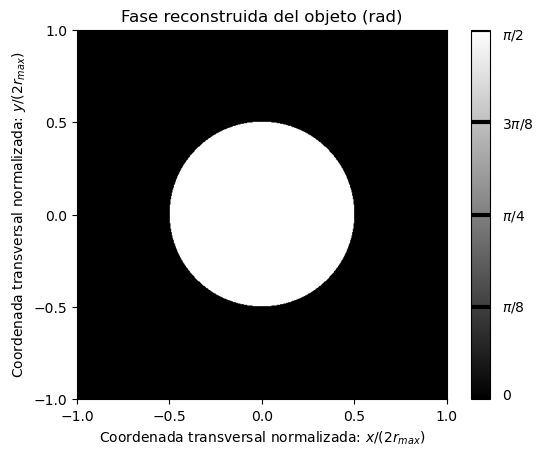
\includegraphics[width=1.1\textwidth,height=1\textwidth]{figure_11.png}
        \caption{}
        \label{f8a}
    \end{subfigure}
    \begin{subfigure}[b]{0.45\textwidth}
        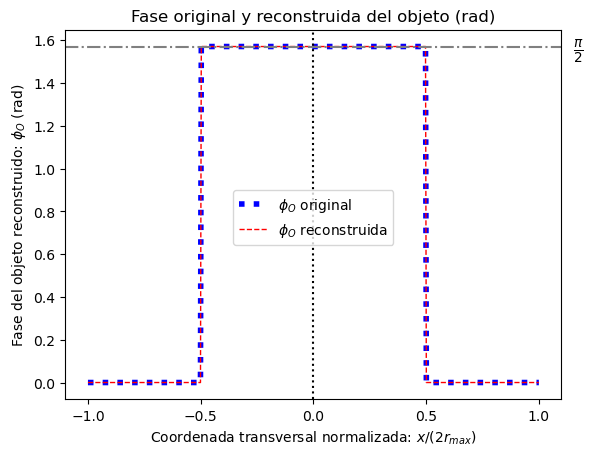
\includegraphics[width=1.2\textwidth,height=1\textwidth]{figure_12.png}
        \caption{}
        \label{f8b}
    \end{subfigure}
    \caption{(a) Disco de fase constante (rad) de $r_{max}=0,5$ sobre un fondo uniforme en el plano del objeto ($z=0$); y (b) perfiles de la fase reconstruida y  de la original para $y = 0$.}
    \label{figura8}
\end{center}
\end{figure}
%%%
vemos como la fase reconstruida de la onda objeto en $z=0$ es una reconstrucción fidedigna de la fase original del objeto. \\ \\
%%%
Ahora,  supongamos que la distribución de amplitud del objeto original es un disco de radio máximo $r_{max}$ con una variación lineal de fase desde el centro de fase $\pi/2$ hasta el borde de fase $0$ sobre un fondo uniforme de fase $0$ y que, al igual que antes, el plano del holograma coincide con el plano objeto. Si seguimos el mismo procedimiento que con el disco de fase constante, tal y como podemos ver  en la Fig.\ref{figura9}, 
%%%
\begin{figure}[b!]
\centering
\begin{center}
    \begin{subfigure}[b]{0.45\textwidth}
    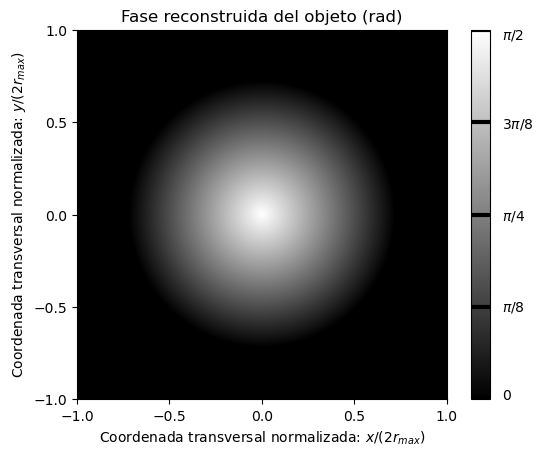
\includegraphics[width=1.1\textwidth,height=1\textwidth]{figure_13.png}
    \caption{}
    \label{f9a}
    \end{subfigure}
    \hspace{10pt}
    \begin{subfigure}[b]{0.45\textwidth}
    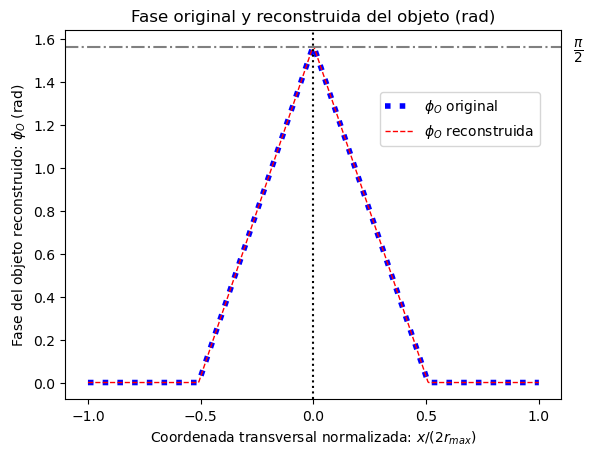
\includegraphics[width=1.2\textwidth,height=1\textwidth]{figure_14.png}
    \caption{}
    \label{f9b}
    \end{subfigure}
    \caption{(a) Variación lineal de un disco de fase (rad) de $r_{max}=0,5$ sobre un fondo uniforme en el plano del objeto ($z=0$);  y (b) perfiles de la fase reconstruida y  de la original para $y = 0$.}
    \label{figura9}
\end{center}
\end{figure}
%%%
conseguiremos reconstruir fielmente la fase original del objeto. Con los resultados obtenidos, podemos verificar que el método de variación de fase es una técnica que consigue reconstruir de forma fidedigna la fase de la distribución de amplitud compleja trasmitida por un objeto cuando el propio plano sobre el que está coincide con el plano de registro del holograma. \\
%%%
En el caso de que el plano del holograma se encuentre a una determinada distancia axial  respecto al plano objeto, será necesario propagar la onda emergente del objeto desde el propio plano sobre el que se encuentra hasta el plano del holograma para llevar a cabo el registro de las intensidades. Tras reconstruir la distribución de amplitud compleja del patrón de difracción del objeto, también será necesario   difractar la onda reconstruida desde el plano del holograma hasta el plano objeto. \\ \\
%%%
Al igual que antes, vamos a suponer que la fase de la distribución de amplitud compleja emergente del objeto es  un disco de  $r_{max}$ de fase constante $\pi /2$ sobre un fondo de fase $0$. Además, supondremos que el plano bidimensional $XY$ sobre el que se encuentra el objeto está a una distancia $z = 500$ mm del plano del holograma.  Para registrar los tres hologramas, primero debemos difractar  la onda trasmitida por el objeto  hasta el plano del holograma.  Después de propagarla hasta  $z = 500$ mm, llevaremos a cabo la etapa de registro del método de variación de fase sobre el patrón de difracción. Si particularizamos para  $\phi_{1} = 0$, $\phi_{2}  = \pi/2$ y $\phi_{3}  = \pi$, registraremos  los hologramas de  la Fig.\ref{f10a},
%%%
\begin{figure}[b!]
\centering
    \begin{subfigure}[b]{0.45\textwidth}
        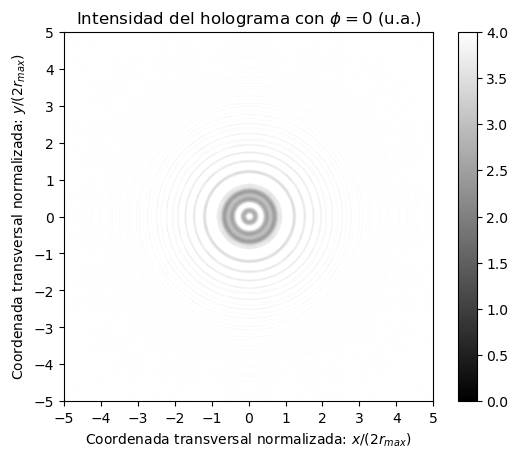
\includegraphics[width=1\textwidth]{figure_15.png}
        \caption{}
        \label{f10a}
    \end{subfigure}
    \begin{subfigure}[b]{0.45\textwidth}
        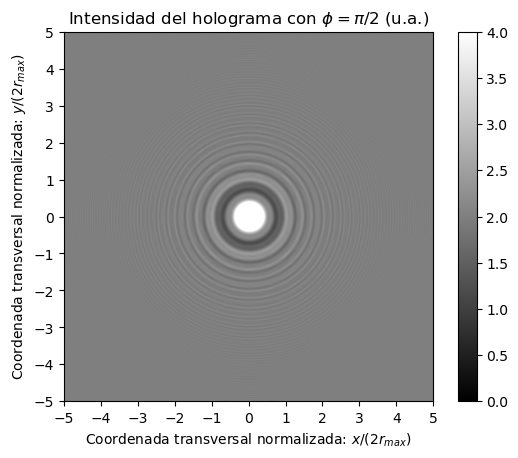
\includegraphics[width=1\textwidth]{figure_16.png}
        \caption{}
        \label{f10b}
        \end{subfigure}
    \begin{subfigure}[b]{0.45\textwidth}
        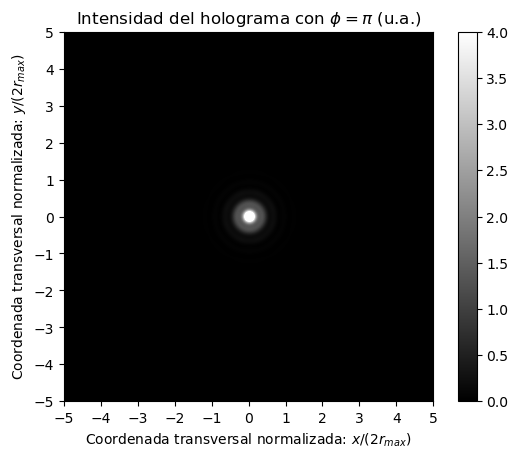
\includegraphics[width=1\textwidth]{figure_17.png}
        \caption{}
        \label{f10c}
    \end{subfigure}
    \begin{subfigure}[b]{0.45\textwidth}
        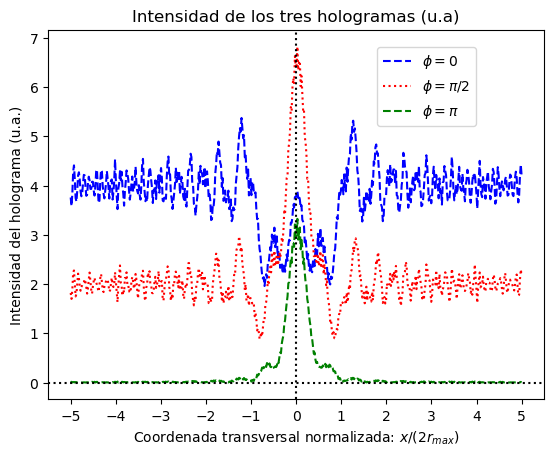
\includegraphics[width=1\textwidth,height=0.87\textwidth]{figure_18.png}
        \caption{}
        \label{f10d}
  \end{subfigure}
  \caption{Intensidad del holograma (u.a.) en eje registrado a una distancia $z = 500$ mm del plano objeto de un disco con $r_{max} = 0,5$ de salto de fase $\pi/2$: (a) con $\phi_1 = 0$; (b) con $\phi_2 = \pi/2$; (c) con $\phi_3 = \pi$; y (d) perfil de los tres hologramas para $y = 0$.}
  \label{figura10}
\end{figure}
%%%
la Fig.\ref{f10b} y  la Fig.\ref{f10c}, respectivamente. Al comparar las imágenes de la Fig.\ref{figura7} con las de la Fig.\ref{figura10}, podemos ver en estas últimas, las franjas interferenciales propias de la difracción.\\ \\
%%%
Una vez hemos registrado las tres intensidades, obtenemos la distribución de amplitud compleja de la Ec.(\ref{Ec.25}) para el patrón de difracción en $z = 500$ mm. Para reconstruir el objeto, debemos llevar a cabo la propagación de Fresnel inversa, es decir, difractaremos el resultado anterior una distancia $ z = -500$ mm desde el plano del holograma hasta el plano propio del objeto. Así,  podremos comparar la fase original de la onda trasmitida por el objeto en el propio plano del objeto con la fase reconstruida en este mismo plano. En la Fig.\ref{figura11}, las comparamos y
%%%
\begin{figure}[b!]
\centering
\begin{center}
    \begin{subfigure}[b]{0.45\textwidth}
        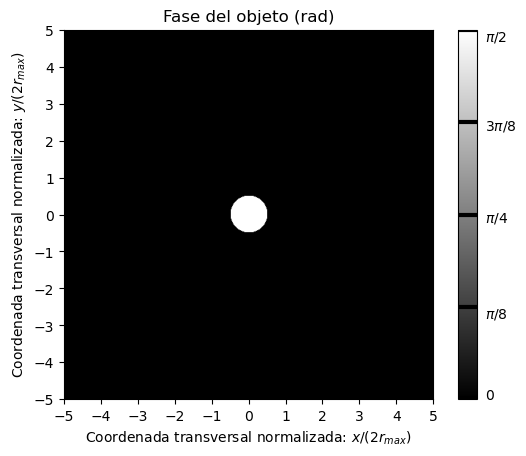
\includegraphics[width=1.1\textwidth,height=1\textwidth]{figure_19.png}
        \caption{}
        \label{f11a}
    \end{subfigure}
    \hspace{10pt}
    \begin{subfigure}[b]{0.45\textwidth}
        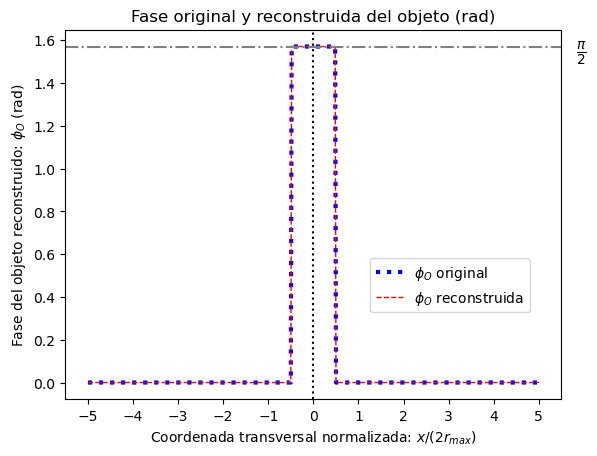
\includegraphics[width=1.2\textwidth,height=1\textwidth]{figure_20.png}
        \caption{}
        \label{f11b}
    \end{subfigure}
  \caption{(a) Disco de fase constante (rad) de $r_{max}=0,5$ sobre un fondo uniforme en el plano del objeto ($z=0$);  y (b) perfiles de la fase reconstruida y  de la original para $y = 0$.}
  \label{figura11}
\end{center}
\end{figure}
%%%
comprobamos que el método de variación de fase es una técnica que reconstruye de manera fidedigna la fase original de la distribución de amplitud compleja emergente del objeto.\\ \\
%%%
Por último, volvemos a considerar que la fase original de la distribución de amplitud compleja emergente del objeto es un disco de radio máximo $r_{max}$ con variación lineal de fase desde el centro $\pi/2$ hasta el borde $0$ sobre un fondo uniforme de fase $0$.  Si el objeto se encuentra a una distancia $z = 500$ mm del plano del holograma, al igual que antes,
%%%
\begin{figure}[t!]
\centering
\begin{center}
    \begin{subfigure}[b]{0.45\textwidth}
        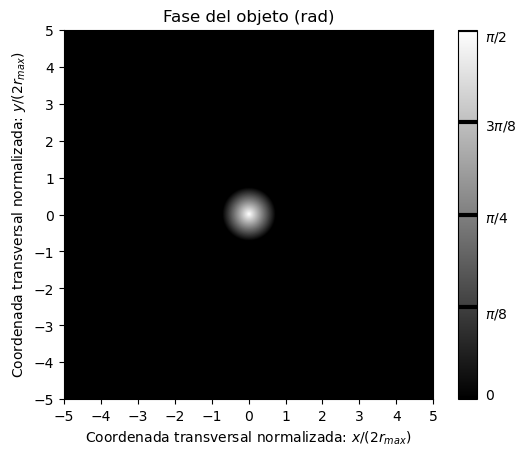
\includegraphics[width=1.1\textwidth,height=1\textwidth]{figure_21.png}
        \caption{}
        \label{f12a}
    \end{subfigure}
    \hspace{15pt}
    \begin{subfigure}[b]{0.45\textwidth}
        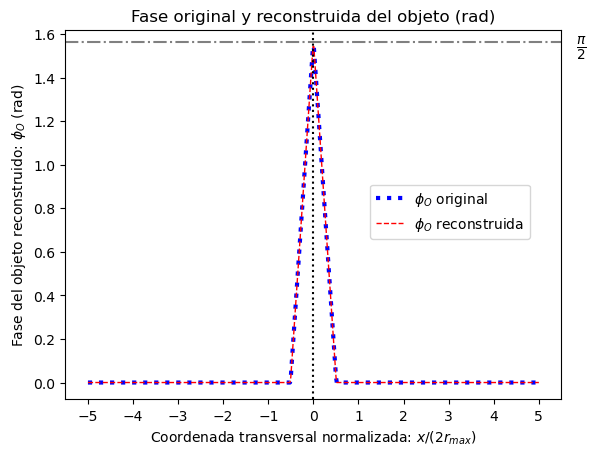
\includegraphics[width=1.2\textwidth,height=1\textwidth]{figure_22.png}
        \caption{}
        \label{f12b}
    \end{subfigure}
    \caption{(a) Variación lineal de un disco de fase (rad) de $r_{max} = 0,5$  sobre un fondo uniforme en el plano del objeto ($z=0$);  y (b) perfiles de la fase reconstruida y  de la original para $y = 0$.}
    \label{figura12}
\end{center}
\end{figure}
%%%
debemos llevar a cabo los pasos que nos llevaron a obtener la Ec.(\ref{Ec.26}). \\ \\
%%%
De nuevo, en la Fig.\ref{figura12}, verificamos que el método de variación de fase es una técnica que permite reconstruir con precisión la fase original de la onda objeto cuando existe una distancia $z$ entre el plano del holograma y el plano del objeto. \\ \\
%%%
Por lo tanto, podemos concluir que el método de variación de fase es un modelo válido que permite recrear fielmente la fase de la distribución de amplitud del objeto en configuraciones en eje, tanto cuando el holograma se registra sobre el plano objeto como si se graba sobre un patrón de difracción. 
%%%%%%%%%%%%%%%%%%%%%%%%%%%%%%
%%% CONCLUSIONES 
%%%%%%%%%%%%%%%%%%%%%%%%%%%%%%
\section{Conclusiones}
Con este trabajo se ha introducido el concepto de la holografía digital. En particular, ha servido para profundizar y entender  el proceso de reconstrucción del campo electromagnético emergente de un objeto, inicialmente desconocido, a partir de provocar su interferencia con un haz de referencia en configuraciones en eje.  \\ \\ 
%%%
En primer lugar, se han presentado y comprendido  los principios teóricos en los que se fundamenta el concepto clásico de la holografía. Después, se ha demostrado que, en la reconstrucción, se forma un halo de luz junto a dos imágenes del objeto, lo que dificulta  al observador la visualización de la imagen reconstruida. Además, se ha comprobado que existe un solapamiento en la reconstrucción de las imágenes  del objeto en configuraciones en eje. Para solucionar el problema del solapamiento, se ha comprendido el porqué es necesario complementar el concepto clásico de holografía  con  la tecnología más actual. Por ese motivo, a continuación, se ha estudiado el concepto de holografía digital y, a partir de él, se han expuesto y desarrollado  las dos técnicas más utilizadas para reconstruir la distribución de amplitud emitida por un objeto. Por un lado, se ha presentado la técnica de filtrado para montajes fuera de eje y por consiguiente, se han expuesto sus limitaciones cuando la banda espectral del objeto  es suficientemente grande o cuando el ángulo interferencial es significativamente pequeño. Por otro lado, se ha expuesto  el método de variación de fase como una técnica efectiva de formación de imágenes cuando la técnica de filtrado no lo es. En concreto, se ha desarrollado para el caso en el que la onda objeto y la onda de referencia interaccionan entre sí de forma cuasi paralela. Además, con la aplicación de estas técnicas, no solo se ha conseguido solucionar  las limitaciones  de la holografía clásica, si no que también se mejora la calidad y la resolución de la imagen reconstruida. Dicho de otro modo, en la reconstrucción de la holografía digital, se consigue eliminar tanto el efecto de la imagen gemela como el halo de luz. Por consiguiente, en este trabajo, se ha comprendido que la holografía digital es una técnica de formación de imágenes que permite recrear una imagen limpia del objeto independientemente del  tipo de configuración. Para finalizar, y  con el fin de comprobar la validez del método de variación de fase en configuraciones en eje, se ha  llevado a cabo la simulación del método para  dos objetos de fase diferentes: uno de fase constante sobre un fondo uniforme  y otro con variación lineal de fase desde el centro hasta el borde. \\ \\ 
%%%
Se puede concluir que la holografía digital es una técnica   que complementa el mecanismo de la holografía clásica con los métodos  digitales más avanzados para el tratamiento de datos. La digitalización de la holografía  permite monitorizar los datos extraídos del holograma,   facilita la aplicación de  métodos numéricos complejos y permite simular computacionalmente tanto la etapa de registro como la etapa de reconstrucción en el ordenador. Por lo tanto, la holografía digital no sufre las restricciones que sí limitaban a la holografía clásica y, además, permite solucionar  la pérdida de información en montajes en eje.
%%%%%%%%%%%%%%%%%%%%%%%%%%%%%%
%%% CONCLUSIONS 
%%%%%%%%%%%%%%%%%%%%%%%%%%%%%%
\section*{Conclusions}
This work has introduced the concept of digital holography. In particular, it has served to deepen and understand the process of reconstructing the emerging electromagnetic field of an object, initially unknown, by causing its interference with a reference beam in on-axis configurations.\\ \\
%%%
First, the theoretical principles underlying the classical concept of holography were presented and understood. Then, it has been shown that, in the reconstruction, a halo of light is formed next to two images of the object. This makes it difficult for the observer to see the reconstructed image. Next, it has been verified that there is an overlap in the reconstruction of the images of the object in configurations on axis. To solve the problem of overlapping, it has been understood why it is necessary to complement the classical concept of holography with the latest technology. For this reason, the concept of digital holography has been studied in the following. The two techniques usually used to reconstruct the amplitude distribution emitted by an object have been presented and developed in this work. On one hand,  the filtering technique for off-axis setups has been presented. Consequently, its limitations have been exposed when the spectral band of the object is sufficiently large or when the interference angle is significantly small. On the other hand, the phase-shifting method has been exposed as an effective imaging technique when the filtering technique is not effective. In particular, it has been developed for the case in which the object wave and the reference wave interact  in quasi-parallel directions.  Moreover, these techniques solve the limitations of classical holography and improves the quality and resolution of the reconstructed image. This is a consequence of eliminate the twin image effect and the light halo that hinders the observation of the image. Therefore, in this work, it has been realised that digital holography is an imaging technique that makes it possible to recreate a good image of the object independently of the type of configuration. Finally, to check the validity of the phase variation method in axis configurations, it has been simulated for two different phase objects: a constant phase disc and a linear variation from centre to edge. \\ \\
%%%
In conclusion, digital holography is a technique that complements the mechanism of classical holography with the most advanced digital methods for data processing. Consequently, digital holography allows the monitoring of data extracted from the hologram, facilitates the application of complex numerical methods and can be used to simulate the registration and reconstruction of an image on the computer. Therefore, it is not limited by the restrictions of the classic holography and allows to solve the loss of information in on-axis configurations.
%%%%%%%%%%%%%%%%%%%%%%%%%%%%%%
%%% REFERENCIAS 
%%%%%%%%%%%%%%%%%%%%%%%%%%%%%%
\addcontentsline{toc}{section}{Referencias}
\bibliographystyle{unsrt}
\bibliography{bibliography.bib}
%%%
\end{document}
%%%%%%%%%%%%%%%%%%%%%%%%%%%%%%
%%% END 
%%%%%%%%%%%%%%%%%%%%%%%%%%%%%%